% !Mode:: "TeX:UTF-8"
%% Thesis Template of Yanshan University
%% for using YSUthesis package with XeLaTeX
% 2012年3月17日
%% 文档参数配置开始:
%%===========================%

\documentclass[]{YSUthesis}
%  showtypeinfo 显示扉页的LaTeX版本信息,去掉即可隐藏版本信息。
%  openany      可以去掉章节起始页必须为奇数页的限制,使章节连续,不出现空白页。
%  推荐的编译顺序为:XeLaTeX > BibTeX > XeLaTeX > XeLaTeX,
%  这样可以生成正确的参考文献和交叉引用链接。

%  设置图形文件的搜索路径。支持图形格式:pdf; png; jpg.
\graphicspath{{chapter/}{figures/}}

%  执行下面的命令可以取消PDF文件中的链接颜色,使用 Adobe Acrobat Reader 查看
%  时,链接可能会有边框,但是在打印时不会出现。
%\hypersetup{colorlinks=false}

% 启用以下这段代码可以让你更改目录的缩进,以备学院有特殊要求。
%\usepackage{titletoc}
%\titlecontents{chapter}[4\ccwd]{}
%                {\bf\contentslabel{4\ccwd}}
%                {\hspace{-4\ccwd}\bf}
%                {\titlerule*[5pt]{.}\contentspage}
%\titlecontents{subsection}[68pt]{}
%                {\contentslabel{40pt}}
%                {\hspace{-4\ccwd}}
%                {\titlerule*[5pt]{.}\contentspage}

% 选择数学字体,xits-math.otf为类Times字体,Cambria Math与Office2010数学公式格式相同。
%\setmathfont{xits-math.otf}


\usepackage{ctex}
\usepackage{subfigure}
\usepackage{bbding}
\usepackage{enumerate}
\usepackage{array}


%%===========================%
%% 文档参数配置结束


%% 文档正式开始
%============================%
\begin{document}


% 以下为封面部分
%----------------------------%
  % 中文封面内容
  \classification{O441.4}                           % 中图分类号
  \UDC{537.8}                                       % UDC
  \title{燕山大学硕士学位论文\LaTeX 模板使用说明}  % 论文题目
  \author{×××}                                      % 作者姓名
  \advisor{×××教授}                                % 导师姓名
  \degree{工程硕士}                                 % 申请学位
  \major{电子信息}                                % 专业
  \institute{电气工程学院}                                % 所在单位
  \defenddate{2023年5月}                        % 答辩日期
  \school{燕山大学}                                 % 院校名称

  % 英文封面内容
  \enstatement{Science}                             % 学科或领域
  \entitle{OPTIMIZATION OF PHOTONIC CRYSTAL FIBER DISPERSION PROPERTIES USING GENETIC ALGORITHM}    % 英文题目
  \enauthor{×××}                                    % 作者英文姓名
  \enadvisor{Professor ×××}                         % 导师英文姓名
  \enschool{Yanshan University}                     % 院校英文名称
  \enathdate{2023.05}                               % 英文答辩日期

  % 生成封面
  \makecover

  % 生成中文封里
  \maketitle

  % 生成英文封里
  \makeenglishtitle

  % 生成原创性声明
  \makelicense


% 以下为前言部分
%----------------------------%
\frontmatter
\pagenumbering{Roman}

  % 摘要
  % !Mode:: "TeX:UTF-8"
\begin{abstract}
xxxxxx

xxxxxx

xxxxxxxxxxxxx

\end{abstract}

\begin{keywords}
xxxx;  xxx;  xxxx 

\end{keywords}

\cleardoublepage

\begin{englishabstract}
xxxxxxxxxxxxxx

xxxxxxxxxxxxxxxx

xxxxxxxxxxxxxxx
\end{englishabstract}

\begin{englishkeywords}
xxx; xxx; xxx
\end{englishkeywords} 

\cleardoublepage

  % 目录
  \tableofcontents
  % 表格目录
  %\listoftables
  % 插图目录
  %\listoffigures

%设置这样字体大小后与word一样了  
\fontsize{11.8pt}\selectfont

% 以下为正文部分
%----------------------------%
\mainmatter
  % !Mode:: "TeX:UTF-8"
\chapter{快速入门}
\label{chap:introduction}

本模板的意义是为了让从未接触过\LaTeX 的新手能尽快的上手,熟悉
本模板的使用。因此本文介绍的大部分内容都将以实例的形式给出,您
可以通过目录快速检索感兴趣的内容。作为一个学文论文作者,你的主
要精力应该是论文的内容而不是论文的格式。字体字号对齐方式是否有
背题图和图注是否在同一页参考文献作者是否缩写期刊名是否缩写——
这些不应该成为一个即将具有硕士学位的人花费大量精力去考虑的问题。
这也是本模板要解决的问题。

本说明的结构安排如下:第\ref{chap:introduction}章是一篇简易教程,完整的示例了论文的
一章可能会遇到的各种问题如插图、公式、图形引用、公式引用和文献
的插入及引用。第\ref{chap:figures}章是关于插图的进阶内容,会涉及到图形的不同排
列形式,图形的大小缩放等。第\ref{chap:table}章是关于表格的内容,涉及如何插入表格,
科技文献常用的三线表以及跨页长表格等问题。第\ref{chap:equ}章是关于公式的进阶内容,涉及公式
的编号、对齐、矩阵和方程组的编写等问题。第\ref{chap:bib}章是关于参考文献,
涉及文献的压缩引用,排序等。第\ref{chap:chap-5}章则介绍了在文章
内加入计算机程序源代码的方法。第\ref{chap:unit}章介绍输入数字和物理量的方法。

\section{高楼大厦始于一砖一瓦}
简单的说,\LaTeX 是一种对文字进行排版处理的程序语言,尽管它的功
能不仅限于此。它与我们常用的Microsoft Word在使用上有较大的区
别。例如我们在MSWord中输入标题时,先输入标题文字,如“绪论”,
然后将其选中,选择MSWord中的“章标题”样式。这是在已经定义好
了章标题样式的前提下。如果从未听说过样式或者没有使用过MSWord样
式的同学,可能会采取更为繁琐的操作,例如分别设定字体,字号,大
纲级别,缩进,对齐方式和自动编号等等。在\LaTeX 中,是这样输入
章标题的:\\[2pt]
\hspace*{5cm}\verb|\chapter{绪论}|\\[2pt]
仅此而已。这里的\verb|\chapter|是一个\textbf{命令},它告诉\LaTeX
“绪论”是章标题,然后\LaTeX 会按照预先定义好的章标题格式来对其
进行处理——这不是我们应该关心的内容。同样,你可以使用
\verb|\section{课题背景}|、\verb|\subsection{理论基础}|和
\verb|\subsubsection{公式推导}|来告诉\LaTeX 这些分别是节标题、
条标题和款标题。\LaTeX 会自动对它们进行格式的设置,并且会自动
为你生成编号。

而图形的插入通常则是通过以下形式:
\begin{verbatim}
\begin{figure}
 
\includegraphics{ysulogo}
\end{figure}
\end{verbatim}
其中ysulogo为插图的文件名,不包含后缀名(\XeLaTeX 支持PDF, PNG, JPG 格式)。与命令不同,这里使用了\\
\verb|\begin{figure}|
和
\verb|\end{figure}|\\
这一对命令来构成一个\textbf{环境}。使用本模板完成学位论文时将会经常
用到命令与环境。一般使用者只要能区分开二者即可,其实只要完成论文的
第一幅插图,后续的插图可以将原来的插图环境复制并稍加修改即可。

\section{一个完整的章节实例}
下边我们使用命令与环境的概念,完成一个迷你章节的例子。

进入YSUthesis文件夹,打开主文件template.tex。进入chapter文件夹,
打开chap-intro.tex文件。该文件对应论文的第一章“绪论”。然后输入如下内容:
\begin{verbatim}
% !Mode:: "TeX:UTF-8"
\chapter{绪论}
我是绪论中的正文文本。

\section{课题背景}
我要使用引用命令为我的文章引用文献:
\ldots加速度为\SI{12345}{\square\micro\meter\per\nano\second},是一般加速度的\num{1.2345e3}倍\supercite{Yablonovitch1987},
误差\SI{+-2e-6}{\square\micro\meter\per\nano\second}。

\subsection{该小节插图}
这里我要使用图形环境插图。注意该插图拥有中英双语图注和自动生成的图形编号。同时我要引用该图形:该图的编号是\ref{fig-pcf}。
\begin{figure}[hptb]
 \centering
 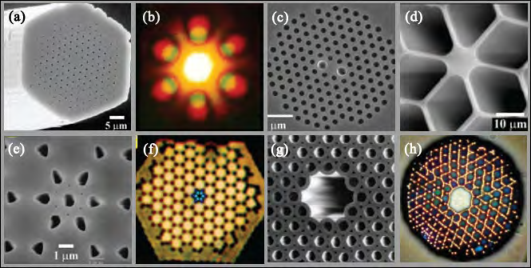
\includegraphics{chp-1_pcf}
 \caption{形式多样的光子晶体光纤。} \label{fig-pcf}
\end{figure}

\subsection{该小节插入公式}
我还要使用公式环境插入公式。注意公式是自动居中编号。同时我也要引用该公式,该公式的编号是\eqref{equ-sample}
\begin{equation}\label{equ-sample}
\sum_{i=1}^n\sin\beta_i^2+\int_a^b\frac{D}{c}\,\mathrm{d}x=0
\end{equation}

\section{本章小结}
以上为本章的所有内容。
\end{verbatim}
保存该文件。切换到template.tex主文件,依次执行菜单``TeX"下的``XeLaTeX" - ``BibTeX" - ``XeLaTeX" - ``XeLaTeX",(这些步骤也可以通过工具栏上的
按钮完成)。之后会在主目录下自动生成PDF文件,您不妨亲自动手试试看!
生成的参考文献如图\ref{fig-ctt}所示。
\begin{figure}[hptb]
 \centering
 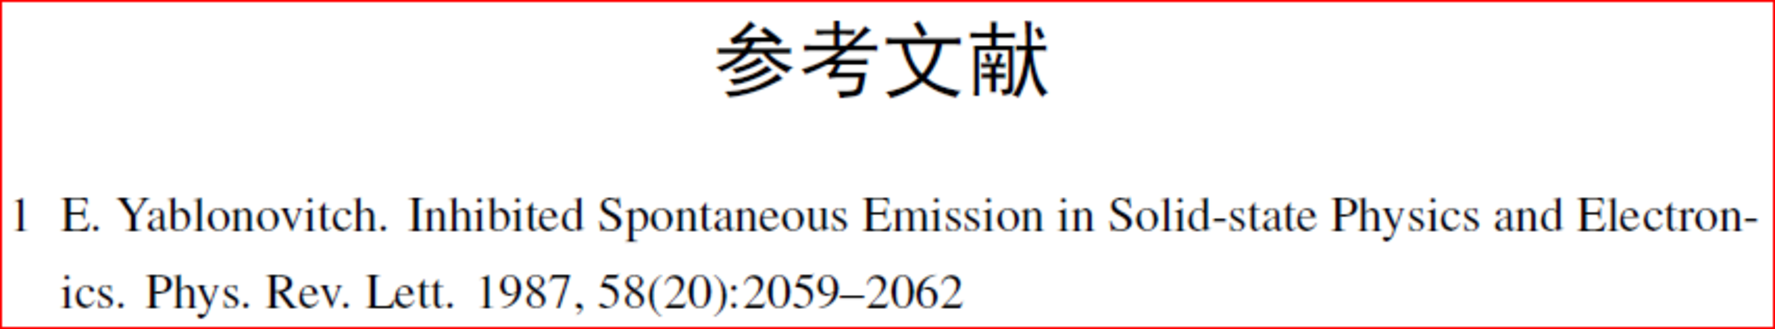
\includegraphics[width=\linewidth]{citation}
\caption{自动生成的参考文献。}\label{fig-ctt}
\end{figure} 
  % !Mode:: "TeX:UTF-8"
\chapter{插图}
\label{chap:figures}

插图主要涉及到:单个居中图形;两个并排图形;两个以上的并排或者堆叠的图形;图题;图形的引用;

\section{单个居中图形}

大多数情况下,需要插入的图形是单个的时候可以使用如下环境:

\begin{verbatim}
\begin{figure}[hptb]
 \centering
 
\includegraphics[width=6cm]{ysulogo}
 \caption{单个居中图形}\label{ysulogo}
\end{figure}
\end{verbatim}

其中的参数“[width=6cm]”指定图形的宽度6 cm。最后的效果如图\ref{ysulogo}所示。
\begin{figure}[hptb]
 \centering
 
\includegraphics[width=6cm]{ysulogo}
 \caption{单个居中图形}\label{ysulogo}
\end{figure}

\section{两个并排图形}
下列代码在文中插入两个并排的图形。它使用了一个称作minipage
的环境。在同一行插入两个并排的minipage,每个minipage包含一
个图形。图中minipage的参数“[0.5$\backslash$linewidth]”指定minipage
的宽度是当前正文页面的0.5倍(一半)。而插图命令中的参数
“[width=$\backslash$textwidth]”则是指定插图的宽度为当前minipage的宽
度。如果这个插图命令是在minipage环境外边的话,参数中的
“$\backslash$textwidth”的宽度为当前正文页面的宽度。
\begin{verbatim}
\begin{figure}[hptb]
  \centering
  \begin{minipage}[t]{0.5\linewidth}
    \centering
    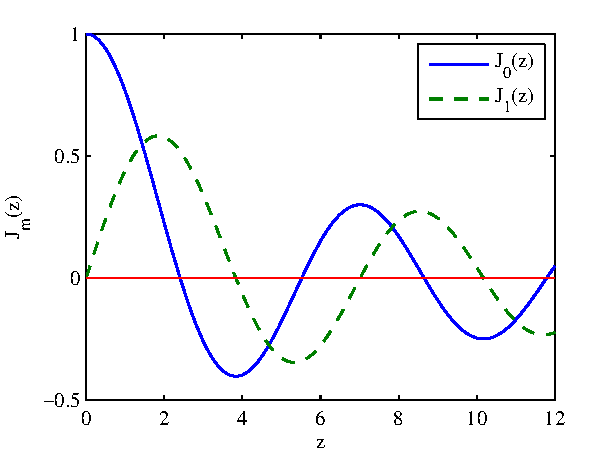
\includegraphics[width=\textwidth]{chp-2_bessel_j}
  \end{minipage}%
  \begin{minipage}[t]{0.5\textwidth}
    \centering
    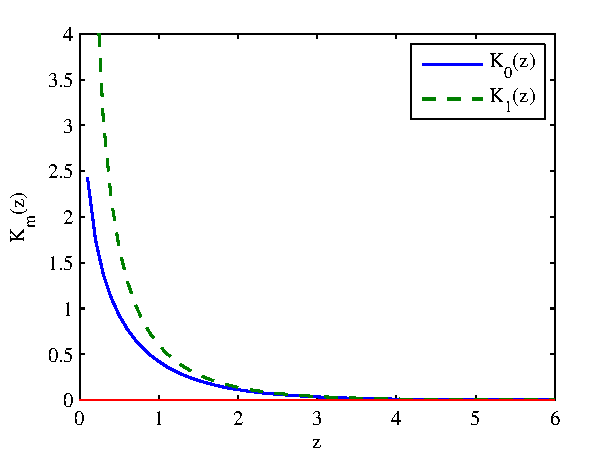
\includegraphics[width=\textwidth]{chp-2_bessel_k}
  \end{minipage}
    \caption{两个并排图形}\label{fig-dbfig}
\end{figure}
\end{verbatim}
最终结果如图\ref{fig-dbfig}所示。
\begin{figure}[hptb]
  \centering
  \begin{minipage}[t]{0.5\linewidth}
    \centering
    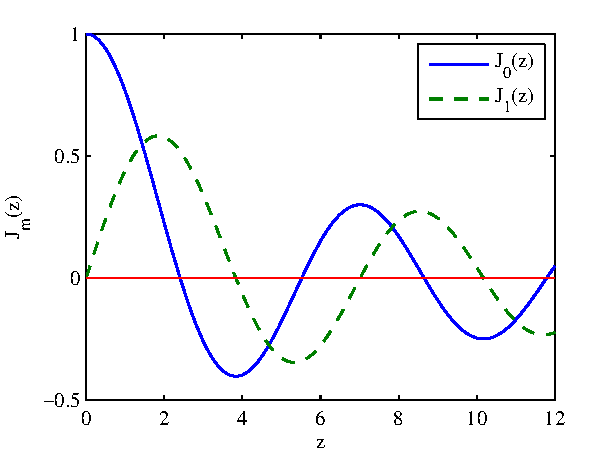
\includegraphics[width=\textwidth]{chp-2_bessel_j}
  \end{minipage}%
  \begin{minipage}[t]{0.5\textwidth}
    \centering
    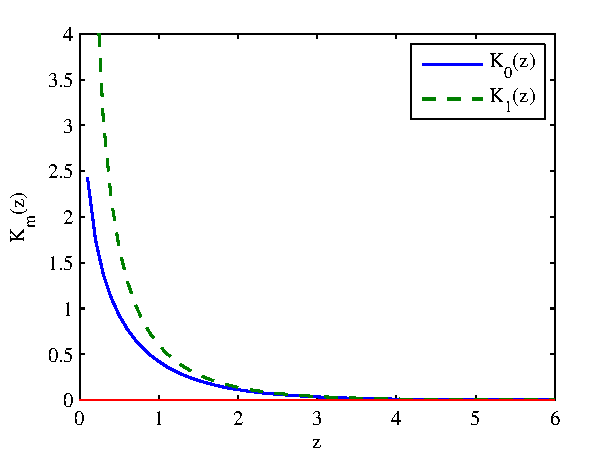
\includegraphics[width=\textwidth]{chp-2_bessel_k}
  \end{minipage}
    \caption{两个并排图形}\label{fig-dbfig}
 \end{figure}

\section{两个以上的并排或者堆叠的图形}
同样是使用minipage的方法,只不过排列的方式不同。例如4幅堆叠排列的图形。
\begin{verbatim}
\begin{figure}[hptb]
  \centering
  \begin{minipage}[t]{0.5\linewidth}
    \centering
    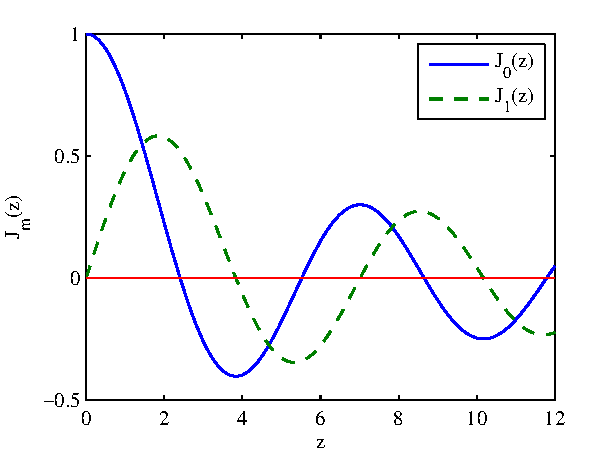
\includegraphics[width=\textwidth]{chp-2_bessel_j}
  \end{minipage}%
  \begin{minipage}[t]{0.5\textwidth}
    \centering
    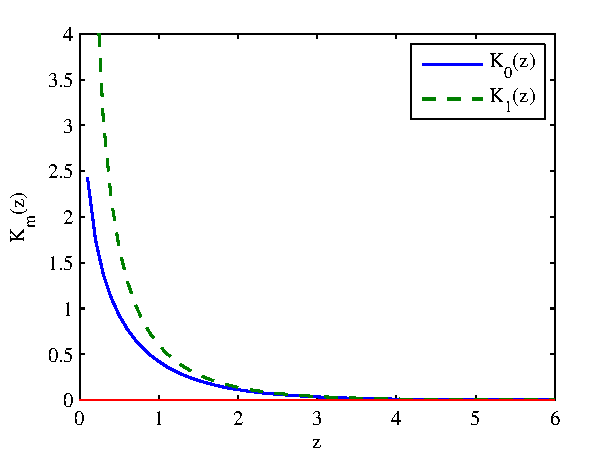
\includegraphics[width=\textwidth]{chp-2_bessel_k}
  \end{minipage}  \\
  \begin{minipage}[t]{0.5\textwidth}
    \centering
    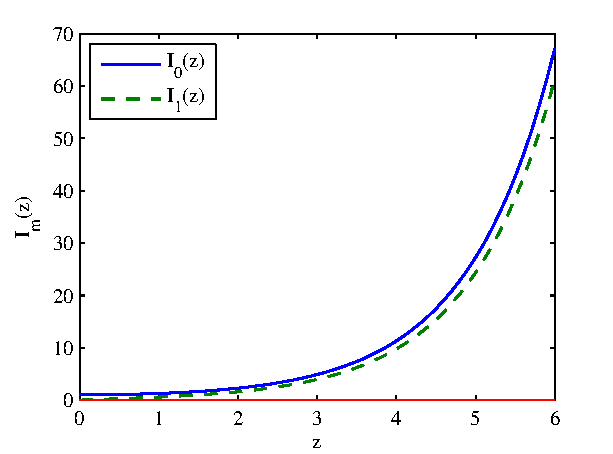
\includegraphics[width=\textwidth]{chp-2_bessel_i}
  \end{minipage}%
  \begin{minipage}[t]{0.5\textwidth}
    \centering
    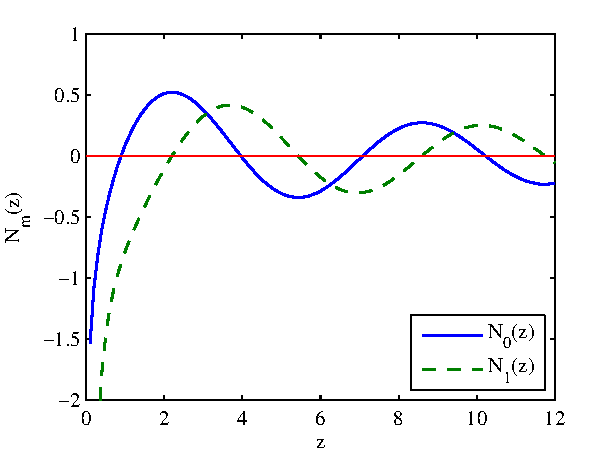
\includegraphics[width=\textwidth]{chp-2_bessel_n}
  \end{minipage}
\caption{贝塞尔函数}  \label{fig-bessel-function}
\end{figure}
\end{verbatim}
注意其中与一对并排图形不同的地方,加入了换行命令“$\backslash\backslash$”。
最终效果如图\ref{fig-bessel-function}所示。
\begin{figure}[hptb]
  \centering
  \begin{minipage}[t]{0.5\linewidth}
    \centering
    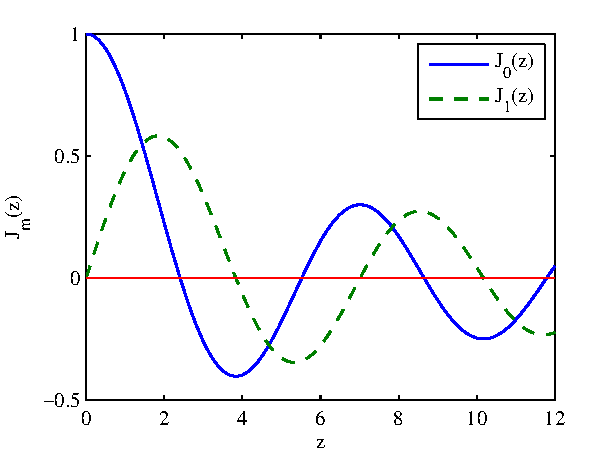
\includegraphics[width=\textwidth]{chp-2_bessel_j}
  \end{minipage}%
  \begin{minipage}[t]{0.5\textwidth}
    \centering
    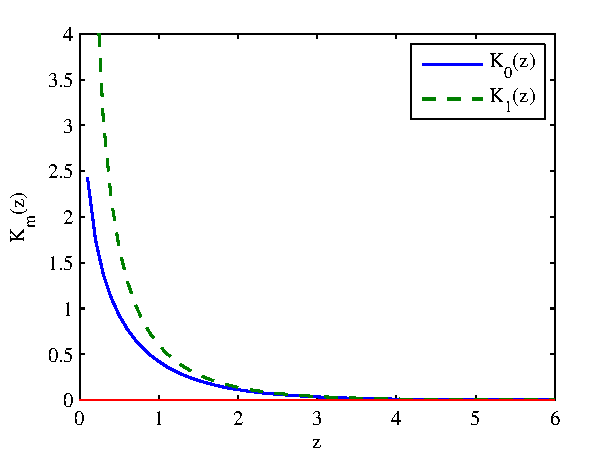
\includegraphics[width=\textwidth]{chp-2_bessel_k}
  \end{minipage}  \\
  \begin{minipage}[t]{0.5\textwidth}
    \centering
    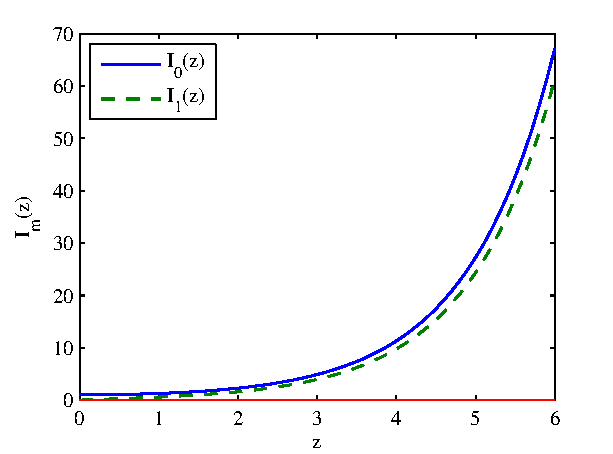
\includegraphics[width=\textwidth]{chp-2_bessel_i}
  \end{minipage}%
  \begin{minipage}[t]{0.5\textwidth}
    \centering
    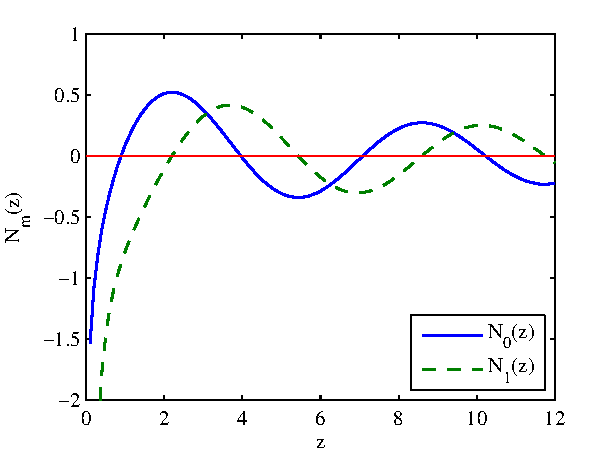
\includegraphics[width=\textwidth]{chp-2_bessel_n}
  \end{minipage}
\caption{贝塞尔函数}  \label{fig-bessel-function}
\end{figure}
其它类似的多个图形并排或者堆叠均可以灵活的运用minipage照猫画虎获得。

\section{图题}
其实上边的例子中已经包含了图题的引用命令\verb|\caption|。
例如图\ref{fig-bessel-function}中:
\begin{verbatim}
    \caption{贝塞尔函数}\label[fig-bessel-function]
\end{verbatim}
为当前的图形添加中文图题“贝塞尔函数”。同时添加标签“fig-bessel-function”。对图形的引用就是通过标签来实现的。

\section{图形的引用}
在已知图形的标签的基础之上,通过命令:
\begin{verbatim}
\ref{label}
\end{verbatim}
来引用标签为“label”的图形。\LaTeX 会自动将其替换为图形的编号。例如:
\begin{verbatim}
贝塞尔函数的图形如图\ref{fig-bessel-function}所示。
\end{verbatim}
的效果如下:\\
贝塞尔函数的图形如图\ref{fig-bessel-function}所示。

  % !Mode:: "TeX:UTF-8"
\chapter{表格}
\label{chap:table}

\section{普通三线表}
科技文献中常用的三线表:
\begin{table}[htbp]
 \centering\zihao{5}
 \caption{燕山大学硕士学位论文参考文献规则}\label{tab:ysubof}
 \begin{tabular}{llr}
 \toprule
    论文版本    & 参考文献标准    & 实施年份(年)  \\
 \midrule
    旧版        & BF7714-87       & 1987            \\
    新版        & GBT7714-2005    & 2005            \\
 \bottomrule
 \end{tabular}
\end{table}

实现代码如下:
\begin{verbatim}
\begin{table}[htbp]
 \centering\zihao{5}
 \caption{燕山大学硕士学位论文参考文献规则}\label{tab:ysubof}
 \begin{tabular}{llr}
 \toprule
    论文版本    & 参考文献标准    & 实施年份(年)  \\
 \midrule
    旧版        & BF7714-87       & 1987            \\
    新版        & GBT7714-2005    & 2005            \\
 \bottomrule
 \end{tabular}
\end{table}
\end{verbatim}

\section{有合并列的三线表}
合并列通常见于表格的第一行,在适当的位置使用\verb|\multicolumn| 命令即可。
\begin{table}[htbp]
\centering\zihao{5}
\caption{带有合并列的三线{\zihao{5}表}}\label{tab:test}
\begin{tabular}{llr} \toprule
\multicolumn{2}{c}{Item} \\ \cmidrule(r){1-2}
Animal & Description & Price (\$)\\ \midrule
Gnat & per gram & 13.65 \\
& each & 0.01 \\
Gnu & stuffed & 92.50 \\
Emu & stuffed & 33.33 \\
Armadillo & frozen & 8.99 \\ \bottomrule
\end{tabular}
\end{table}


该表格是采用如下代码实现的:
\begin{verbatim}
\begin{table}[htbp]
 \centering
 \caption{三线表}\label{tab:test}
 \begin{tabular}{llr}
 \toprule
    \multicolumn{2}{c}{Item}            \\
 \cmidrule(r){1-2}
    Animal  & Description   & Price (\$)\\
 \midrule
    Gnat    & per gram      & 13.65     \\
            & each          & 0.01      \\
    Gnu     & stuffed       & 92.50     \\
    Emu     & stuffed       & 33.33     \\
    Armadillo & frozen      & 8.99      \\
 \bottomrule
 \end{tabular}
\end{table}
\end{verbatim}

\section{表格的引用}
表格的引用同样是使用\verb|\ref{}| 命令实现的。例如“表\verb|\ref{tab:ysubof}|” 输出的结果为:表\ref{tab:ysubof}

  % !Mode:: "TeX:UTF-8"
\chapter{公式}
\label{chap:equ}
本章介绍基本公式的输入方法;矩阵和向量的输入;方程组的输入;多行公式的换行与对齐。
\LaTeX 中数学公式的输入依赖于数学环境。

在正文中用到的简短公式,可以直接使用两个美元符号“\$”括起来,如:
\begin{verbatim}
直角三角形三边长度满足关系式$a^2+b^2=c^2$
\end{verbatim}
得到的结果是:\\
直角三角形三边长度满足关系式$a^2+b^2=c^2$\\

而对于一些较为重要或者较复杂、需要编号的公式,则需要使用各种数学环境,例如使用equation环境:
\begin{verbatim}
\begin{equation}\label{chp-mode}
\mathbfit{E}=\mathrm{Re}(\mathbfit{E}(\mathbfit{r}))e^{j\omega t}
\end{equation}
\end{verbatim}
得到的结果是:
\begin{equation}\label{chp-mode}
\mathbfit{E}=\mathrm{Re}(\mathbfit{E}(\mathbfit{r}))e^{j\omega t}
\end{equation}
对它的引用方式为:\verb|公式\eqref{chp-mode}|\\
得到的结果为:公式\eqref{chp-mode}

如果不想对公式进行编号,则可以使用equation*环境:
\begin{verbatim}
\begin{equation*}\label{chp-m2}
\mathbfit{E}=\mathrm{Re}(\mathbfit{E}(\mathbfit{r}))e^{j\omega t}
\end{equation*}
\end{verbatim}
得到的结果是:
\begin{equation*}\label{chp-m2}
\mathbfit{E}=\mathrm{Re}(\mathbfit{E}(\mathbfit{r}))e^{j\omega t}
\end{equation*}

\section{上下标}
\verb|a_1+b^2\times c_1^2=0|输出结果为:$a_1+b^2\times c_1^2=0$

\section{分式}
命令\verb|\frac, \dfrac\ tfrac|可以用来输出分式:
\begin{verbatim}
\begin{equation}\label{fr}
  \sin\dfrac{\cos\dfrac{a}{b}}{c}=
  \sin\frac{\cos\frac{a}{b}}{c}=
  \sin\tfrac{\cos\tfrac{a}{b}}{c}
\end{equation}
\end{verbatim}
输出的结果是:
\begin{equation}\label{fr}
\sin\dfrac{\cos\dfrac{a}{b}}{c}=
\sin\frac{\cos\frac{a}{b}}{c}=
\sin\tfrac{\cos\tfrac{a}{b}}{c}
\end{equation}

当使用括号来括起纵向尺寸较大的对象例如分式时,要使用\verb|\left| 和
\verb|\right| 命令使括号在纵向上伸长。例如:
\begin{verbatim}
\begin{equation}\label{frr}
  \left(\frac{a}{b}\right)=(\frac{a}{b})
\end{equation}
\end{verbatim}
的输出结果是:
\begin{equation}\label{frr}
\left(\frac{a}{b}\right)=(\frac{a}{b})
\end{equation}

\section{矢量点乘与叉乘}
矢量点乘:\verb|$\mathbfit{A}\cdot\mathbfit{B}$|输出:$\mathbfit{A}\cdot\mathbfit{B}$

矢量叉乘:\verb|$\mathbfit{C}\times\mathbfit{D}$|输出:$\mathbfit{C}\times\mathbfit{D}$

\section{求和与积分}
命令\verb|\sum|和命令\verb|\int|负责输出求和与积分号。例如:
\begin{verbatim}
\begin{equation}\label{equ-sum}
  \sum_{i=1}^n\sin\beta_i^2=0
\end{equation}
\end{verbatim}
输出结果为:
\begin{equation}\label{equ-sum}
\sum_{i=1}^n\sin\beta_i^2=0
\end{equation}
\begin{verbatim}
\begin{equation}\label{equ-int}
  \int_a^b\frac{c}{d}\,\mathrm{d}x=0
\end{equation}
\end{verbatim}
输出结果为:
\begin{equation}\label{equ-int}
  \int_a^b\frac{c}{d}\,\mathrm{d}x=0
\end{equation}


\section{矩阵与数组}
矩阵与数组使用array环境:
\begin{verbatim}
\begin{equation}\label{equ-array}
  \left(
    \begin{array}{c} a \\ c \end{array}
  \right)=
  \left(
    \begin{array}{cc} a & b \\ c & d \end{array}
  \right)
\end{equation}
\end{verbatim}
输出结果是:
\begin{equation}\label{equ-array}
  \left(
  \begin{array}{c} a \\ c \end{array}
  \right)=
  \left(
  \begin{array}{cc} a & b \\ c & d \end{array}
  \right)
\end{equation}
也可以使用matrix环境:
\begin{verbatim}
\begin{equation}\label{equ-matrix}
  \begin{matrix} 0 & 1 \\ 1 & 0\end{matrix}=
  \begin{pmatrix}0 &-i \\ i & 0\end{pmatrix}=
  \begin{bmatrix}1 & 0 \\ 0 &-1\end{bmatrix}=
  \begin{vmatrix}a & b \\ c & d\end{vmatrix}
\end{equation}
\end{verbatim}
输出结果是:
\begin{equation}\label{equ-matrix}
  \begin{matrix} 0 & 1 \\ 1 & 0\end{matrix}=
  \begin{pmatrix}0 &-i \\ i & 0\end{pmatrix}=
  \begin{bmatrix}1 & 0 \\ 0 &-1\end{bmatrix}=
  \begin{vmatrix}a & b \\ c & d\end{vmatrix}
\end{equation}

\section{多行公式与对齐方法}
多行公式排列,每个公式都有自己的编号通常使用align环境。例如:
\begin{verbatim}
\begin{align}
  a_1+a_2+a_3 &=0 \label{equ-s1}\\
  b_1+b_2+b_3+b_4 &=0 \label{equ-s2}\\
  c_1+c_2 &=0 \label{equ-v1}
\end{align}
\end{verbatim}
输出结果为:
\begin{align}
  a_1+a_2+a_3 &=0 \label{equ-s1}\\
  b_1+b_2+b_3+b_4 &=0 \label{equ-s2}\\
  c_1+c_2 &=0 \label{equ-v1}
\end{align}
其中符号“\&”为对齐符号。这里实现了等号对齐。

\section{带有大括号的方程组}
与多行公式不同,方程组左侧使用“\verb|\left{|”加了一个大括号,另外只有一个公式编号,因此采用equation和aligned结合的方式,例如:
\begin{verbatim}
\begin{equation}\label{equ-fml}
  \left\{
  \begin{aligned}
    x^2+y^2 &=0\\
    x+y+z^2 &=0\\
    x^2+y+z &=0
  \end{aligned}
  \right.
\end{equation}
\end{verbatim}
输出结果为:
\begin{equation}\label{equ-fml}
  \left\{
  \begin{aligned}
    x^2+y^2 &=0\\
    x+y+z^2 &=0\\
    x^2+y+z &=0
  \end{aligned}
  \right.
\end{equation}


  % !Mode:: "TeX:UTF-8"
\chapter{参考文献}
\label{chap:bib}

所有被引用的参考文献信息均存储在模板目录中的“bib”目录下,文件名为“tex.bib”。
由于使用了BibTeX,参考文献的格式是不需要手动调整。模板中的ysubst.bst文件负责
文献格式输出。这里推荐您使用软件JabRef 来对文献进行管理。JabRef 支持中文,它可
以在这个网址下载到。\url{http://jabref.sourceforge.net/}

首先需要了解一个概念叫“BibTeX key”,也称作“BibTeX键”。它可以简单的理解为一篇
参考文献的“身份证号”。每一篇参考文献均有一个属于自己的不会重复的BibTeX key。
在引用文献的时候,需要使用引用命令\verb|\supercite{}|。

\section{单一参考文献}
例如这里我引用一篇文献:
\begin{verbatim}
P.Russell 是光子晶体光纤之父\supercite{Knight1996}
\end{verbatim}
其中“Knight1996”是我要引用的文献的BibTeX 键。输出的结果为:\\[5pt]
 P.Russell 是光子晶体光纤之父\supercite{Knight1996}\\[5pt]
 注意文献的编号是自动生成的,并且具有超链接功能。单击编号可以定位到文末的参考文献章节。

\section{多个连续参考文献}
 如果要一次引用多个文献,只要在引用命令中用英文逗号隔开各个BibTeX键即可,例如:
 \begin{verbatim}
我要引用2 篇文献\supercite{Knight1996,Knight2000}
\end{verbatim}
输出结果为: \\[5pt]
我要引用2 篇文献\supercite{Knight1996,Knight2000}


如果是3 篇或者以上,加入更多BibTeX 键即可。例如:
 \begin{verbatim}
3 篇文献\supercite{Knight1996,Knight2000,Knight2002}
\end{verbatim}
输出结果为: \\[5pt]
3 篇文献\supercite{Knight1996,Knight2000,Knight2002}

更多文献的例子:
 \begin{verbatim}
很多很多文献\supercite{Kivshar2008,John1987,Jing2010,Jeon2005,%
Jastrow2008,Jackson2008,Huttunen2005,Hou2008,Hilligsoe2004,%
Hassani2008,Han2002}
\end{verbatim}

输出的结果为:很多很多文献\supercite{Kivshar2008,John1987,Jing2010,Jeon2005,%
Jastrow2008,Jackson2008,Huttunen2005,Hou2008,Hilligsoe2004,%
Hassani2008,Han2002}



\section{多个不连续参考文献}
 \begin{verbatim}
四个不连续文献\supercite{Zhu2004,Zhu2001,Yin2011,Knight1996}
\end{verbatim}
四个不连续文献\supercite{Zhu2004,Zhu2001,Yin2011,Knight1996}

  % !Mode:: "TeX:UTF-8"
\chapter{插入程序代码}
\label{chap:chap-5}

使用lisitings宏包可以在正文中插入程序的代码,插入的代码有自己的字体,可以实现行号、关键字高亮等功能。该环境的参数language决定了程序
的类型,例如\verb|language={[77]Fortran}|指定程序代码为FORTRAN语言;\verb|language={MATLAB}|指定程序代码为MATLAB的m语言。下边给出具体的例子。

\section{FORTRAN}
\begin{verbatim}
\begin{lstlisting}[language={[77]Fortran},
numbers=left,
numberstyle=\tiny,
basicstyle=\small\ttfamily,
stringstyle=\color{purple},
keywordstyle=\color{blue}\bfseries,
commentstyle=\color{brown},
frame=single]
C MATLAB gateway
      subroutine mexFunction(nlhs, plhs, nrhs, prhs)
C variables
      integer nlhs, nrhs
      integer plhs(*), prhs(*)
C input pointers
      pr_x=mxgetpr(prhs(1))
      pr_x1=mxgetpr(prhs(2))
C output pointers
      plhs(1)=mxCreateDoubleScalar(0)
      pr_y=mxGetPr(plhs(1))
C calculation
      call eim(%val(pr_x),%val(pr_x1),%val(pr_y))
      end subroutine mexFunction
\end{lstlisting}
\end{verbatim}
输出的结果为:
\begin{lstlisting}[language={[77]Fortran},
numbers=left,
numberstyle=\tiny,
basicstyle=\small\ttfamily,
stringstyle=\color{purple},
keywordstyle=\color{blue}\bfseries,
commentstyle=\color{brown},
frame=single]
C MATLAB gateway
      subroutine mexFunction(nlhs, plhs, nrhs, prhs)
C variables
      integer nlhs, nrhs
      integer plhs(*), prhs(*)
C input pointers
      pr_x=mxgetpr(prhs(1))
      pr_x1=mxgetpr(prhs(2))
C output pointers
      plhs(1)=mxCreateDoubleScalar(0)
      pr_y=mxGetPr(plhs(1))
C calculation
      call eim(%val(pr_x),%val(pr_x1),%val(pr_y))
      end subroutine mexFunction
\end{lstlisting}

\section{MATLAB}
\begin{verbatim}
\begin{lstlisting}[language={MATLAB},
numbers=left,
numberstyle=\tiny,
basicstyle=\small\ttfamily,
stringstyle=\color{purple},
keywordstyle=\color{blue}\bfseries,
commentstyle=\color{brown},
frame=single]
% bessel j

n=-0:0.1:12;
y=n*0;
b0n=besselj(0,n);
b1n=besselj(1,n);
plot(n,b0n,'-',n,b1n,'-',0:0.1:12,y)

ylabel('J_m(z)')
xlabel('z')
legend('J_0(z)','J_1(z)')
\end{lstlisting}
\end{verbatim}
输出的结果为:
\begin{lstlisting}[language={MATLAB},
numbers=left,
numberstyle=\tiny,
basicstyle=\small\ttfamily,
stringstyle=\color{purple},
keywordstyle=\color{blue}\bfseries,
commentstyle=\color{brown},
frame=single]
% bessel j

n=-0:0.1:12;
y=n*0;
b0n=besselj(0,n);
b1n=besselj(1,n);
plot(n,b0n,'-',n,b1n,'-',0:0.1:12,y)

ylabel('J_m(z)')
xlabel('z')
legend('J_0(z)','J_1(z)')
\end{lstlisting}

\section{C++}
\begin{verbatim}
\begin{lstlisting}[language={C++},
numbers=left,
numberstyle=\tiny,
basicstyle=\small\ttfamily,
stringstyle=\color{purple},
keywordstyle=\color{blue}\bfseries,
commentstyle=\color{brown},
frame=single]
# include{iostream.h}
void main()
int r;
double n;
{
cout<<"hello, LaTeX!"<<endl;
}
\end{lstlisting}
\end{verbatim}
输出的结果为:
\begin{lstlisting}[language={C++},
numbers=left,
numberstyle=\tiny,
basicstyle=\small\ttfamily,
stringstyle=\color{purple},
keywordstyle=\color{blue}\bfseries,
commentstyle=\color{brown},
frame=single]
# include{iostream.h}
void main()
int r;
double n;
{
cout<<"hello, LaTeX!"<<endl;
}
\end{lstlisting}

  % !Mode:: "TeX:UTF-8"
\chapter{数字物理量与单位}
\label{chap:unit}
模板加载了siunitx 宏包,可以实现长串数字位数的正确分割和各种物理量单位的自动格式化,避免
手工调用数学环境输入单位。尤其适用于理工科各种物理量的输入。该宏包的引入主要是为了解决论文
格式标准中的这个要求:
数字的书写不必每格一个数码,一般每两数码占一格,数字间分节不用分位号",",\emph{凡4位或4位以上的数都从个位起每3位数空\textbf{半个数码(1/4汉字)}。“\num{3 000000}”,不要写成}“3,000,000”,\emph{小数点后的数从小数点起向右按\textbf{每三位一组分节}。一个用阿拉伯数字书写的多位数不能从数字中间转行。}

\section{数字}
使用\verb|\num| 命令可以输入正确格式的长数字,包括科学计数法格式的数字。

\begin{table}[htbp]
\centering\zihao{5}
\caption{siunitx 宏包与\LaTeX 数学环境输出效果对比}
\begin{tabular}{ll|ll}
\toprule
siunitx 输出样式    & siunitx 输入方式          & \LaTeX 数学环境输出样式  & \LaTeX 数学环境输入方式     \\
\midrule
\num{123456789}     & \verb|\num{123456789}|    & 123456789             & \verb|123456789|         \\
\num{-1000000}      & \verb|\num{-1000000}|     & $-1000000$            & \verb|$-1000000$|        \\
\num{3.2e-8}        & \verb|\num{3.2e-8}|       & $3.2\times 10^{-8}$   & \verb|$3.2\times 10^{-8}$|\\
\num{1.2345678}     & \verb|\num{1.2345678}|    & 1.2345678             & \verb|1.2345678|          \\
\bottomrule
\end{tabular}
\end{table}

\section{单位}
单独输入单位时,可以采用\verb|\si|命令。

\begin{table}[htbp]
\centering\zihao{5}
\caption{单位的不同输入方式}
\begin{tabular}{ll}
\toprule
输出样式  &输入方式     \\
\midrule
\si{kg.m/s^2}                           & \verb|\si{kg.m/s^2}|         \\
\si{g_{polymer}mol_{cat}.s^{-1}}       & \verb|\si{g_{polymer}mol_{cat}.s^{-1}}|\\
\si{\kilo\gram\metre\per\square\second} & \verb|\si{\kilo\gram\metre\per\square\second}|\\
\si{\gram\per\cubic\centi\metre}        &\verb|\si{\gram\per\cubic\centi\metre}|\\
\si{\square\volt\cubic\lumen\per\farad} &\verb|\si{\square\volt\cubic\lumen\per\farad}|\\
\si{\metre\squared\per\gray\cubic\lux}  &\verb|\si{\metre\squared\per\gray\cubic\lux}|\\
\si{\henry\second}                      &\verb|\si{\henry\second}|\\
\bottomrule
\end{tabular}
\end{table}

\section{同时输入数字与单位}

通常情况下,数字与单位是共同给出的,这时可以采用\verb|\SI| 命令。注意这里的 SI 是大写的。并且加入不同的可选项,最终的效果也不同。

\begin{table}[htbp]
\centering\zihao{5}
\caption{同时输入数字与单位}
\begin{tabular}{ll}
\toprule
输出样式    & 输入方式  \\
\midrule
\SI[mode=text]{1.23}{J.mol^{-1}.K^{-1}}         & \verb|\SI[mode=text]{1.23}{J.mol^{-1}.K^{-1}}| \\
\SI{.23e7}{\candela}                            & \verb|\SI{.23e7}{\candela}|\\
\SI[per-mode=symbol]{1.99}[\$]{\per\kilogram}   & \verb|\SI[per-mode=symbol]{1.99}[\$]{\per\kilogram}|\\
\SI[per-mode=fraction]{1,345}{\coulomb\per\mole}& \verb|\SI[per-mode=fraction]{1,345}{\coulomb\per\mole}|\\
\bottomrule
\end{tabular}
\end{table}

\section{附1:国际标准单位与导出单位输入方式}

\begin{table}[htbp]
\centering\zihao{5}
\caption{国际标准单位输入方式}
\begin{tabular}{lllp{10pt}lll}
\toprule
单位    & 命令  & 符号  &   & 单位    & 命令  & 符号  \\
\midrule
安培    & \verb|\ampere|    & \si{\ampere}   && 坎德拉  & \verb|\candela|   & \si{\candela}  \\
开尔文  & \verb|\kelvin|    & \si{\kelvin}   && 千克    & \verb|\kilogram|  & \si{\kilogram}    \\
米      & \verb|\meter|     & \si{\meter}    && 摩尔    & \verb|\mole|      & \si{\mole}    \\
秒      & \verb|\second|    & \si{\second}   &&     &        &      \\
\bottomrule
\end{tabular}
\end{table}

\begin{table}[htbp]
\centering\zihao{5}
\caption{国际标准导出单位输入方式}
\begin{tabular}{lllp{10pt}lll}
\toprule
单位    & 命令  & 符号  &   & 单位    & 命令  & 符号  \\
\midrule
becquerel       & \verb|\becquerel|     & \si{\becquerel}       & & newton      & \verb|\newton|    & \si{\newton} \\
degree Celsius  & \verb|\degreeCelsius| & \si{\degreeCelsius}   & & ohm         & \verb|\ohm|       & \si{\ohm}\\
coulomb         & \verb|\coulomb|       & \si{\coulomb}         & & pascal      & \verb|\pascal|    & \si{\pascal}\\
farad           & \verb|\farad|         & \si{\farad}           & & radian      & \verb|\radian|    & \si{\radian} \\
gray            & \verb|\gray|          & \si{\gray}            & & siemens     & \verb|\siemens|   & \si{\siemens}    \\
hertz           & \verb|\hertz|         & \si{\hertz}           & & sievert     & \verb|\sievert|   & \si{\sievert}\\
henry           & \verb|\henry|         & \si{\henry}           & & steradian   & \verb|\steradian| & \si{\steradian}\\
joule           & \verb|\joule|         & \si{\joule}           & & tesla       & \verb|\tesla|     & \si{\tesla}\\
katal           & \verb|\katal|         & \si{\katal}           & & volt        & \verb|\volt|      & \si{\volt}\\
lumen           & \verb|\lumen|         & \si{\lumen}           & & watt        & \verb|\watt|      & \si{\watt}\\
lux             & \verb|\lux|           & \si{\lux}             & & weber       & \verb|\weber|     & \si{\weber}\\
\bottomrule
\end{tabular}
\end{table}
\section{附2:国际标准单位前缀}

\begin{table}[htbp]
\centering\zihao{5}
\caption{国际标准单位前缀输入方式}
\begin{tabular}{llllp{10pt}llll}
\toprule
名称    & 命令          & 符号          & 指数  &   & 名称      & 命令          & 符号      & 指数 \\
\midrule
yocto   & \verb|\yocto| & \si{\yocto}   & -24   &   & deca      &\verb|\deca|   &\si{\deca} & 1     \\
zepto   & \verb|\zepto| & \si{\zepto}   & -21   &   & hecto     &\verb|\hecto|  &\si{\hecto}& 2\\
atto    & \verb|\atto|  & \si{\atto}    & -18   &   & kilo      &\verb|\kilo|   &\si{\kilo} & 3\\
femto   & \verb|\femto| & \si{\femto}   & -15   &   & mega      &\verb|\mega|   &\si{\mega} & 6\\
pico    & \verb|\pico|  & \si{\pico}    & -12   &   & giga      &\verb|\giga|   &\si{\giga} & 9\\
nano    & \verb|\nano|  & \si{\nano}    & -9    &   & tera      &\verb|\tera|   &\si{\tera} & 12\\
micro   & \verb|\micro| & \si{\micro}   & -6    &   & peta      &\verb|\peta|   &\si{\peta} & 15\\
milli   & \verb|\milli| & \si{\milli}   & -3    &   & exa       &\verb|\exa|    &\si{\exa}  & 18\\
centi   & \verb|\centi| & \si{\centi}   & -2    &   & zetta     &\verb|\zetta|  &\si{\zetta}& 21\\
deci    & \verb|\deci|  & \si{\deci}    & -1    &   & yotta     &\verb|\yotta|  &\si{\yotta}& 24\\
\bottomrule
\end{tabular}
\end{table}

  % !Mode:: "TeX:UTF-8"
\begin{conclusion}
\label{chap:conclusion}

结论作为学位论文正文的组成部分,单独排写,不加章标题序号,不标注引用文献。结论内容一般在2000字以内。

结论应是作者在学位论文研究过程中所取得的创新性成果的概要总结,不能与摘要混为一谈。结论应包括论文的主要结果、创新点、展望三部分,在结论中应概括论文的核心观点,明确、客观地指出本研究内容的创新性成果(含新见解、新观点、方法创新、技术创新、理论创新),并指出今后进一步在本研究方向进行研究工作的展望与设想。对所取得的创新性成果应注意从定性和定量两方面给出科学、准确的评价,分(1)、(2)、(3)…条列出,宜用“提出了”、“建立了”等词叙述。此外,结论的撰写还应符合以下基本要求:

(1)结论具有相对的独立性,不应是对论文中各章小结的简单重复。结论要与引言相呼应,以自身的条理性、明确性、客观性反映论文价值。对论文创新内容的概括,评价要适当。

(2)结论措辞要准确、严谨,不能模棱两可,避免使用“大概”、“或许”、“可能是”等词语。结论中不应有解释性词语,而应直接给出结果。结论中一般不使用量的符号,而宜用量的名称。

(3)结论应指出论文研究工作的局限性或遗留问题,如条件所限,或存在例外情况,或本论文尚难以解释或解决的问题。

(4)常识性的结果或重复他人的结果不应作为结论。

\end{conclusion} 

  %% 附录
  %\appendix
  %
\chapter{Ñàɽ´óѧÑо¿ÉúѧλÂÛÎÄ׫д¹æ·¶}
\label{chap:requires}

\begin{equation}
a=b^2+c_2
\end{equation}

ѧλÂÛÎÄÊÇÑо¿Éú¿ÆѧÑо¿¹¤×÷µÄÈ«Ãæ×ܽᣬÊDZíÊöÆäÑо¿³É¹û¡¢´ú±íÆäÑо¿Ë®Æ½µÄÖØҪѧÊõÎÄÏ××ÊÁÏ£¬ÊÇÉêÇëºÍÊÚÓèÏàӦѧλµÄ»ù±¾ÒÀ¾Ý¡£×«Ð´Ñ§Î»ÂÛÎÄÊÇÑо¿ÉúÅàÑøµÄ»ù±¾ÑµÁ·Ö®Ò»£¬±ØÐë°´Õչ淶ÈÏÕæÖ´ÐС£Ö¸µ¼½ÌʦӦ¼ÓÇ¿Ö¸µ¼£¬Ñϸñ°Ñ¹Ø¡£
\begin{figure}[htbp]
\centering

\includegraphics[width=8cm]{ysulogo}
\caption{The Yanshan University LOGO}
\end{figure}
׫дµÄÂÛÎÄÓ¦·ûºÏ¹ú¼Ò¼°×¨Òµ²¿ÃÅÖƶ¨µÄÓйرê×¼£¬·ûºÏººÓïÓï·¨¹æ·¶¡£

˶ʿºÍ²©Ê¿Ñ§Î»ÂÛÎijýѧÊõˮƽ²»Í¬Í⣬ËüÃǵÄ׫дҪÇó»ù±¾Ò»Ö¡£

\section{·âÃ棨·âÒ»¡¢·âƤ£©}

²Î¼û¸½Â¼1ѧλÂÛÎÄ·âÃæʾÀý¡£

·âÃæ¸ñʽ²ÎÕÕ¸½Â¼1¡£¸÷ÏîÃû³ÆµÄºáÏòλÖÃÓ¦¾ÓÖа²ÅÅ£¬ÊúÏò¼ä¾à°´¸½Â¼1°²ÅÅ¡£

¿ª±¾³ß´ç£¬²©Ê¿ÂÛÎĵÄΪA4£¬×°¶©ÇÐÆëºóΪ205¡Á290mm£»Ë¶Ê¿ÂÛÎĵÄΪB5£¬×°¶©ÇÐÆëºóΪ178¡Á250£¬µ¥Î»Îªmm¡£

²©Ê¿ÂÛÎĵÄÊé¼¹´¦Ó¦Ó¡£ºÂÛÎÄÌâÄ¿£¨Ð¡3ºÅºÚÌ壬¾àÉϱßÏß50mm£©¡¢ÐÕÃû£¨¾àϱßÏß30 mm£©¡£

\section{·âÀ·â¶þ£©}

²©Ê¿¡¢Ë¶Ê¿Ñ§Î»ÂÛÎĵķâÀï°üÀ¨ÖÐÎÄÒ³¼°Ó¢ÎÄÒ³¡£ÖС¢Ó¢ÎÄÒ³µÄ°æʽÏàͬ¡£¶ÔÓÚ²©Ê¿¡¢Ë¶Ê¿µÈ²»Í¬Çé¿öÕßµÄѧλÂÛÎÄ·âÀï¿É²Î¿¼¸½Â¼2¡£

ÒÔÑо¿Éú±ÏҵͬµÈѧÁ¦ÉêÇëѧλÕߣ¬ÐèÔÚ·âÀïµÄÓÒÉϽǼÓÉÏÈçÏÂ×ÖÑù£º£¨Í¬µÈѧÁ¦ÈËÔ±£©¡£

\section{ÕªÒª¼°¹Ø¼ü´Ê}

ÕªÒªÊÇѧλÂÛÎĵıØÒª¸½¼Ó²¿·Ö£¬ÊÇÒÔÌṩѧλÂÛÎÄÄÚÈݹ£¸ÅΪĿµÄ£¬²»¼ÓÆÀÂۺͲ¹³ä½âÊÍ£¬¼òÃ÷¡¢È·ÇмÇÊöѧλÂÛÎÄÖØÒªÄÚÈݵÄÍêÕû¶ÌÎÄ¡£Ëü·´Ó³ÁËѧλÂÛÎĵľ«»ª¡£ÕªÒªÓ¦ÒÔŨËõµÄÐÎʽ¸ÅÀ¨Ñ§Î»ÂÛÎÄÑо¿¹¤×÷µÄÄ¿µÄ¡¢¿ÎÌâ¡¢»ù±¾¹Ûµã¡¢Ö÷ÒªÄÚÈÝ¡¢Ñо¿·½·¨¼°½áÂ۵ȡ£ÕªÒªÓ¦¾ßÓжÀÁ¢ÐÔºÍ×ÔÃ÷ÐÔ£¬²¢ÓµÓÐÓëѧλÂÛÎÄͬµÈÁ¿µÄÖ÷ÒªÐÅÏ¢£¬¼´²»ÔĶÁѧλÂÛÎÄÈ«ÎľÍÄÜ»ñµÃ±ØÒªµÄÐÅÏ¢¡£

²©Ê¿¼°Ë¶Ê¿Ñ§Î»ÂÛÎĵÄÕªÒª¾ùÒªÇóÓÃÖС¢Ó¢Á½ÖÖÎÄ×Ö¸ø³ö£¬ÖÐÎÄÔÚÇ°¡£

ÕªÒªµÄ×ÖÊý£¬ÒÔºº×ּƣ¬Ë¶Ê¿Ñ§Î»ÂÛÎÄΪ500¡«650×Ö£»²©Ê¿Ñ§Î»ÂÛÎÄΪ900¡«1200×Ö¡£ÕªÒªÒ³²»Ð´ÂÛÎÄÌâÄ¿¡£ÕªÒªÖв»ÒËʹÓù«Ê½¡¢Í¼±í¼°²Î¿¼ÎÄÏ×ÐòºÅ¡£

ÕªÒªÒ³µÄÆäËüÒªÇó¼û¸½Â¼3ÕªÒª¼°¹Ø¼ü´ÊʾÀý¡£

¹Ø¼ü´ÊÊÇΪÁËÊÊÓ¦¼ÆËã»ú×Ô¶¯¼ìË÷µÄÐèÒª£¬´ÓÂÛÎÄÖÐÑ¡È¡µÄÄܹ»·´Ó³ÎÄÏ×ÌØÕ÷ÄÚÈݵĹ淶ÐÔ´Ê£¨³ÆÐð´Ê»òÖ÷Ìâ´Ê£©¡£Ó¦°´GB3860-83¡¶ÎÄÏ×Ö÷Ìâ±êÒý¹æÔò¡·µÄ¹æ¶¨Ñ¡È¡¡£¶ÔÓÚÄÇЩ·´Ó³ÐÂѧ¿Æ¡¢Ð¼¼ÊõÖеÄÖØÒªÊõÓҲ¿É×÷Ϊ¹Ø¼ü´Ê±ê³ö¡£¹Ø¼ü´ÊÒ»°ãÁÐ5¡«10¸ö£¬°´´ÊÌõÍâÑÓ²ã´Î´Ó´óµ½Ð¡ÅÅÁС£

\section{ѧλÂÛÎĵÄ×é³É²¿·ÖºÍÅÅÁÐ˳Ðò}

ѧλÂÛÎÄÒ»°ãÓÉÒÔϼ¸¸ö²¿·Ö×é³É£º·âÃæ¡¢ÂÛÎÄÕªÒª¡¢ÂÛÎÄĿ¼¡¢ÕýÎÄ¡¢²Î¿¼ÎÄÏס¢
·¢±íÎÄÕÂĿ¼¡¢ÖÂлµÈ¡£

\section{Ŀ¼}

²©Ê¿Ñ§Î»ÂÛÎÄĿ¼ÓÃÖС¢Ó¢Îĸø³ö£¬Ë¶Ê¿Ñ§Î»ÂÛÎÄĿ¼ֻÓÃÖÐÎĸø³ö¡£Ä¿Â¼Ò³µÄÆäËüÒªÇó¼û¸½Â¼4Ŀ¼ʾÀý¡£

\section{ÕýÎÄ}

\subsection{ÕýÎĵÄÄÚÈÝ}

ÕýÎÄÓÉÐ÷ÂÛ¡¢±¾ÂۺͽáÂÛÈý²¿·Ö×é³É¡£

\subsubsection{Ð÷ÂÛ}

Ð÷ÂÛÊÇѧλÂÛÎÄÖ÷Ì岿·ÖµÄ¿ª¶Ë£¬ÊÇȫƪÂÛÎĵÄÒý×Ó¡£Ð÷ÂÛÖ÷Òª»Ø´ð"ΪʲôÑо¿£¨Why£©"Õâ¸öÎÊÌâ¡£ËüÖ÷Òª°üÀ¨£º

(1)Ñо¿µÄ³ö·¢µãÓëÄ¿µÄ£»

(2)Ñо¿µÄÖ÷ÒªÎÊÌâ¼°·¶Î§£¬¼´Ñо¿Ö÷Ìâ¼ò½é£»

(3)ÓëѧλÂÛÎÄÓйصÄÖØÒªÎÄÏ××ÊÁÏ×ÛÊö£¬Ïà¹ØÁìÓòÇ°È˼°ËûÈËÑо¿³É¹û¡¢Ë®Æ½ºÍ֪ʶ¿Õ°×£¬´æÔÚµÄÖ÷ÒªÎÊÌâÒÔ¼°¼±´ý½â¾öºÍÍêÉƵÄÎÊÌ⣻

(4)ÀíÂÛ·ÖÎöÒÀ¾Ý£¬Ñо¿ÉèÏ룬Ñо¿·½·¨ºÍʵÑéÉè¼ÆµÄ¸ÅÊö£»

(5)Ô¤ÆÚÑо¿½á¹û£¬¿ÆѧÒâÒåºÍʵÓüÛÖµ¡£

ΪÁË˵Ã÷ѧλÂÛÎÄ×÷Õ߶ÔÑо¿·½°¸µÄ³ä·ÖÂÛÖ¤£¬·´Ó³×÷ÕßÔÚÏà¹ØµÄѧ¿ÆÁìÓòÖдﵽµÄѧʶˮƽÒÔ¼°¾ßÓпªÀ«µÄ¿ÆѧÊÓÒ°£¬Í¨³£½«ÎÄÏ××ÛÊö×÷ΪÐ÷ÂÛµÄÖØÒªÄÚÈÝ¡£

×ÛÊöÓôóÁ¿Æª·ù¶Ô±¾Ñо¿¿ÎÌâ½øÐÐÀúÊ·»Ø¹Ë£¬¶ÔÇ°È˺ÍËûÈ˵ÄÑо¿¹¤×÷¼°³É¹û½øÐÐ×ÛºÏÆÀÊö£¬È»ºóÒý³ö×Ô¼ºµÄ¿ÎÌâÑо¿ÄÚÈÝ¡£×ÛÊöÏ൱ÓÚÔÚѧλÂÛÎÄÑо¿ÁìÓòÄÚ½øÐÐÒ»´ÎÐÅÏ¢×ÊÁϵÄרÌâÑо¿±¨¸æ¡£Ëü·´Ó³ÁËÑо¿ÉúÔĶÁÓйØÖø×÷¡¢Ñ§ÊõÆÚ¿¯ºÍÎÄÏ××ÊÁϵÄÇé¿ö£»Ò²·´Ó¦ËûËù¾ß±¸µÄ»ù´¡ºÍרҵ֪ʶÒÔ¼°¶ÀÁ¢µÄ×ÔѧÄÜÁ¦¡£×ÛÊöÒªÇóÑо¿Éú¶ÔËùÔĶÁµÄÎÄÏ××ÊÁϽøÐÐÏû»¯¡¢·ÖÎö¡¢ÅжϺÍ×ۺϣ¬¾ö¶¨È¡Éᣬȷ¶¨×Ô¼ºËùÓ¦¿ªÕ¹¿ÆÑй¤×÷µÄÄÚÈÝ¡£Ö»ÓÐÔÚÈÏÕæϸÖ²éÔIJο¼ÎÄÏ׵Ļù´¡ÉÏ£¬²ÅÄÜʹ×Ô¼ºµÄÑо¿Ñ¡Ìâ¾ßÓпɿ¿µÄ»ù´¡£¬¾¡Á¿±ÜÃâÖظ´Ç°È˵ÄÑо¿¹¤×÷£¬´Ó¶øÔÚÇ°È˵Ļù´¡ÉϽâ¾öÇ°ÈËûÓнâ¾ö»òÓдýÍêÉƵŤ×÷¡£

׫дѧλÂÛÎĵÄÐ÷ÂÛʱ£¬²»ÒªÓëÕªÒªÀ×ͬ£¬²»ÒªÚ¹ÊÍ»ù±¾ÀíÂÛ£¬²»ÒªÍƵ¼»ù±¾¹«Ê½£¬²»Òª½éÉÜÑо¿·½·¨Ï¸½Ú¡£Ð´·¨Ó¦¿ªÃżûɽ£¬ÑÔ¼òÒâê࣬´ë´Ê¾«Á¶¡£

\subsubsection{±¾ÂÛ}

±¾ÂÛÊÇÂÛÎĵÄÖ÷Ì岿·Ö£¬ÊÇ×÷ÕßÑо¿³É¹ûµÄչʾºÍ±íÊö¡£Ö÷Òª»Ø´ð"ÔõôÑо¿£¨how£©"Õâ¸öÎÊÌâ¡£ËüÕë¶ÔÐ÷ÂÛ²¿·ÖÌá³öµÄÂ۵㣬ȫÃæ͸³¹µÄ½øÐзÖÎöÂÛÖ¤£¬³ä·Ö±í´ï×÷Õߵļû½â¡£ÖÐÐÄÂÛµãµÄÂÛÖ¤¿ÉÒÔ´Ó²»Í¬µÄ½Ç¶ÈÕ¹¿ª£¬Òò´Ë£¬¿É½¨Á¢²»Í¬µÄ·ÖÂ۵㣬¹²Í¬Î§ÈÆÖÐÐÄÂÛµãΪÆä·þÎñ¡£

±¾ÂÛÔÚ°²ÅŲã´ÎÉÏÖ÷ÒªÓÐÈýÖÖ·½·¨£º¢ÙµÝ½øʽ£¬¼´ÏÈÌá³öÒ»¸öÂ۵㣬Ȼºó²½²½ÉîÈ룬²ã²ãÕ¹¿ª£¬Ñ­Ðò½øÐÐÂÛÊö£»¢Ú²¢ÁÐʽ£¬¼´°ÑÖÐÐÄÂÛµãµÄ¼¸¸ö´ÓÊôÂ۵㲢ÁÐÆðÀ´£¬·Ö±ð¼ÓÒÔÂÛÊö¡£¢Û½áºÏʽ£¬¼´°ÑµÝ½øʽºÍ²¢ÁÐʽ½áºÏÔÚÒ»ÆðʹÓã¬ÕâÖÖ·½Ê½¶àÓÃÓÚÄÚÈݽ϶ࡢƪ·ù½Ï³¤µÄѧλÂÛÎÄ¡£²ã´Î¿ÉÓÃС±êÌâ»òÐòÂë±íʾ¡£

±¾ÂÛµÄÂÛÖ¤·½·¨Ö÷ÒªÓУº¹éÄÉ·ÖÎö·¨¡¢ÑÝÒï·ÖÎö·¨¡¢ÀýÖ¤·¨¡¢ÒýÖ¤·¨¡¢¶¯Òò·ÖÎö·¨¡¢±È½Ï·ÖÎö·¨¡¢ÒòËØ·ÖÎö·¨¡¢×ÛºÏÆÀÎö·¨µÈ£¬¿ÉÊÓÇé¿öÁé»îÑ¡Óá£

±¾ÂÛͨ³£Õ¼Ñ§Î»ÂÛÎĵĴ󲿷Öƪ·ù¡£ËüµÄ¾ßÌå³ÂÊö·½Ê½ÍùÍù²»Í¬Ñ§¿ÆÓнϴóµÄ²î±ð£¬²»ÄÜǣǿµØ×÷³öͳһµÄ¹æ¶¨¡£Ò»°ãÓ¦ÔÚÂÛÎÄ×ÜÌå¿ò¼ÜÏ°´"¸ÅÄîµÄÌá³ö£¬ÀíÂÛµÄÂÛÖ¤£¬·½·¨µÄÑ¡Ôñ£¬ÊÔÑéµÄ¹Û²ì£¬Êý¾ÝµÄ´¦ÀíÓë·ÖÎö£¬½á¹ûµÄ¼ìÑé"µÈ£¬Öð²ã·ÖÎö£¬·ÖÕÂ׫д¡£Ã¿Ò»ÕµÄ×îºó¶¼ÒªÓÐ"±¾ÕÂС½á"¡£±¾ÕÂС½áÊÇÓÃʵ¼ùºÍÊý¾Ý¸ø³öµÄ·ÖÎöÑо¿½á¹û£¬×î¼ÉÖ÷¹ÛÍƲâ³É·Ö¡£
±¾
ÂÛÒªÇó˼·ÇåÎú£¬ºÏºõÂß¼­£¬ÓÃÓï¼ò½à׼ȷ¡¢Ã÷¿ìÁ÷³©£»ÄÚÈÝÎñÇó¿Í¹Û¡¢¿Æѧ¡¢Í걸£¬Òª¾¡Á¿ÈÃÊÂʵºÍÊý¾Ý˵»°¡£·²ÊÇÓüòÒªµÄÎÄ×ÖÄܹ»½²Çå³þµÄÄÚÈÝ£¬Ó¦ÓÃÎÄ×Ö³ÂÊö¡£ÓÃÎÄ×Ö²»ÈÝÒ×˵Ã÷°×»ò˵ÆðÀ´±È½Ï·±ËöµÄ£¬Ó¦Óñí»òͼÀ´³ÂÊö¡£Êý¾ÝµÄÒýÓÃÒªÑϽ÷È·ÇУ¬×ÊÁϵÄÒýÓÃÒª±êÃ÷³ö´¦¡£

½Ì¿ÆÊéʽµÄ׫д·½·¨ÊÇ׫дѧλÂÛÎĵĵÚÒ»´ó¼É¡£¶ÔÒÑÓеÄ֪ʶ±ÜÃâÖØÐÂÃèÊöºÍÂÛÖ¤£¬¾¡Á¿²ÉÓñê×¢²Î¿¼ÎÄÏ׵ķ½·¨£»¶ÔÓõ½µÄijЩÊýѧ¸¨×ôÊֶΣ¬Ó¦·ÀÖ¹¹ý·Ö×¢Òâϸ½ÚµÄÊýѧÍÆÑÝ£¬ÐèҪʱ¿É²ÉÓø½Â¼µÄÐÎʽÊÕÈëѧλÂÛÎĹ©¶ÁÕßÑ¡ÔÄ¡£

\subsubsection{½áÂÛ}

½áÂÛÊÇָѧλÂÛÎÄ×îÖÕµÄ×ÜÌå½áÂÛ¡£Ö÷Òª»Ø´ð"Ñо¿³öʲô£¨what£©"Õâ¸öÎÊÌâ¡£ËüÊÇÔÚ¶Ô±¾ÂÛ·ÖÎö¡¢×ۺϵĻù´¡É϶ÔÈ«ÎĵÄ×ܽáºÍÉý»ª£¬ÊǶÔÐ÷Âۺͱ¾ÂÛÂÛµãµÄºôÓ¦£¬ÊǶÔÈ«ÎĵĻ­Áúµã¾¦µÄÊÕÊø£¬Ò²ÊǶԱ¾ÂÛÖи÷ÕÂС½áµÄÔÙ×ۺϡ£¿ÉÒÔ×÷Ϊ½áÂÛµÄÖ÷ÒªÄÚÈÝÓУº

£¨1£©	±¾¿ÎÌâµÄÀíÂÛ¡¢·½·¨¡¢Éè¼Æ¼ÆËãºÍÊÔÑéÑо¿½á¹ûµÈµÄ¹éÄɺÍ×ܽ᣻

£¨2£©	Ã÷È·»Ø´ð±¾Ñо¿¿ÎÌâËùÌá³öµÄÎÊÌâºÍÈÎÎñ½â¾öµÄ³Ì¶ÈºÍÈ¡µÃµÄ½øÕ¹£»

£¨3£©	Ã÷È·Ö¸³ö±¾Ñо¿ÄÚÈݵĴ´ÔìÐԳɹû»ò´´ÐµãÀíÂÛ£¨º¬Ð¹۵㡢ÐÂ˼·¡¢Ð¼û½â£©ºÍ·½·¨£»

£¨4£©	¶ÔÑо¿³É¹ûÓ¦ÓÃÇ°¾°ºÍÉç»á¡¢¾­¼Ã¼ÛÖµµÈ¼ÓÒÔÔ¤²âºÍÆÀ¼Û£»

£¨5£©	Ö¸³ö½ñºóÔÚ±¾Ñо¿·½Ïò½øÒ»²½¿ªÕ¹Ñо¿¹¤×÷µÄÉèÏë¡¢Õ¹ÍûºÍ½¨Ò飬ÒÇÆ÷É豸µÄ¸Ä½ø£¬Éдý½â¾öµÄÎÊÌâ¡£

׫д½áÂÛʱӦעÒâµÄÊÂÏ

£¨1£©	½áÂÛÓ¦¸ÃÃ÷È·¡¢¾«Á¶¡¢ÍêÕû¡¢×¼È·¡¢´ë´ÇÑÏÃÜ£¬²»º¬ºýÆä´Ê£»

£¨2£©	½áÂÛÒªÒ»·ÖΪ¶þ£¬Òª×ðÖØÇ°È˵ÄÑо¿³É¹û£¬ÊµÊÂÇóÊǵÄÆÀ¼Û×Ô¼ºµÄ³É¹û£¬ÇÐÎðÑÔ¹ýÆäʵ£¬ÔÚÎÞ³ä·ÖµÄ°ÑÎÕʱ£¬Ó¦¸ÃÁôÓÐÓàµØ¡£

£¨3£©	½áÂÛÓ¦·´Ó³×Ô¼º´ÓÊÂÑо¿¹¤×÷È¡µÃµÄ³É¼¨£¬ÊôÓÚÇ°ÈË»òËûÈËÒÑÓеÄÕýÈ·½áÂÛ£¬Ó¦²»Ìá»ò¾¡Á¿ÉÙÌá¡£

½áÂÛÓ¦·ÖÌõ׫д£¬×ÖÊýÒ»°ã²»¶àÓÚ2000×Ö¡£


\subsection{ÕýÎĵÄ׫дҪÇó}

\subsubsection{ѧλÂÛÎÄ×ÖÊý}

²©Ê¿Ñ§Î»ÂÛÎÄÕýÎÄ×ÖÊý£¬Àí¹¤¿ÆΪ8¡«12Íò×Ö£»¹ÜÀí¼°ÈËÎÄѧ¿ÆΪ10¡«14Íò×Ö£¬ÆäÖÐÐ÷ÂÛÕ¼Ò»Íò×Ö×óÓÒ¡£

˶ʿѧλÂÛÎÄÕýÎÄ×ÖÊý£¬Àí¹¤¿ÆΪ4¡«6Íò×Ö£¬¹ÜÀíѧ¿Æ5¡«7Íò×Ö£¨MBA3¡«4Íò×Ö£¬°¸Àý·ÖÎöÂÛÎIJ»ÉÙÓÚ2Íò×Ö£©£¬ÈËÎÄѧ¿ÆΪ3¡«5Íò×Ö£¬Íâ¹úÓïѧ¿Æ²»ÉÙÓÚ2ÍòÍâÎÄ´Ê¡£ÆäÖÐÐ÷ÂÛ£¨ÈËÎÄѧ¿ÆΪ"µ¼ÑÔ"£¬Íâ¹úÓïѧ¿ÆΪ"ÒýÑÔIntroduction"£©Õ¼3000¡«5000×Ö¡£

\subsubsection{ѧλÂÛÎĵİæÃæÒªÇó}

(1) ҳü

ҳüӦ¾ÓÖÐÖÃÓÚÒ³ÃæÉϲ¿¡£µ¥ÊýҳüµÄÎÄ×ÖΪ"Õ¼°±êÌâ"£»Ë«ÊýҳҳüµÄÎÄ×ÖΪ"Ñàɽ´óѧ˶ʿ£¨²©Ê¿£©Ñ§Î»ÂÛÎÄ"¡£Ò³Ã¼µÄÎÄ×ÖÓÃ5ºÅËÎÌ壨ÎÄ×ÖÉÏ¿ÕÒ»ÐÐÊéд£©¡£Ò³Ã¼ÎÄ×ÖÏÂÃæΪÁ½ÌõºáÏß(Á½ÌõºáÏߵij¤¶ÈÓë°æо³ß´çÏàͬ£¬Ë¶Ê¿ÂÛÎÄÏß´Ö0. 5°õ£¬²©Ê¿ÂÛÎÄÏß´Ö1.5°õ£©¡£

(2) Ò³Âë

ÕªÒªºÍĿ¼µÄÒ³ÂëÓÃÂÞÂíÊý×Ö£¬ÕýÎĵÄÒ³ÂëÓð¢À­²®Êý×Ö£¬¾ÓÖбêÓÚÒ³Ãæµ×²¿¡£ÕýÎIJ¿·ÖµÄÊ×Ò³ºÍ·­¿ªºóµÄÿһÓÒÒ³¶¼Ó¦¸ÃÊǵ¥ÊýÒ³Âë¡£Ñо¿ÉúѧλÂÛÎĵÄÔ­¼þÒªÇóÓüÆËã»úÅÅ°æ¡¢±à¼­Óë´òÓ¡£¬ÓàÕ߿ɸ´Ó¡¡£

(3) ÕýÎIJã´Î±àÅÅ

½¨Òé²ÉÓñí1Ëùʾ¸ñʽ£¬µ«Èô½ÚÏÂÃæÎÞÐèÁÐÌõÕßÒ²¿ÉÖ±½ÓÁпî»òÏî¡£

Õ±êÌâÓÃС2ºÅºÚÌå×Ö£¬ºáÏò¾ÓÖÐÅÅ·Å£¬ÊúÏòλÖÃÓëĿ¼ҳҳÌâÉÏ¡¢ÏÂÁô¿ÕÏàͬ£¬ÌâÐòÓëÌâÃû¼äÁôÒ»×Ö¿Õ¡£

½Ú±êÌâÓÃС3ºÅºÚÌ壬Ìõ±êÌâÓÃ4ºÅºÚÌ壬¿î±êÌâÓÃС4ºÅºÚÌ壬ÕýÎÄÓÃС4ºÅËÎÌå×Ö¡£

Íâ¹úÓïѧ¿ÆÂÛÎÄӦʹÓÃÓ¢ÎÄTimes New RomanС4ºÅÌ壬²»¿ÉʹÓû¨Ìå×Ö£»ÊéÃû¡¢ÎÄÏ×ÃûµÈ×÷Æ·Ãû³ÆӦʹÓÃбÌå×Ö£¬¶ÎÂäÊéд²ÉÓÃÊ×ÐÐËõ½ø¸ñʽ¡£

¸÷²ã´Î±êÌâ¾ù²»µÃÖÃÓÚÒ³ÃæµÄ×îºóÒ»ÐУ¬¼´²»ÔÊÐí"±³Ìâ"¡£

²©Ê¿Ñ§Î»ÂÛÎÄ¿ª±¾ÎªA4£¬Ò³±ß¾àΪÉèÖãºÉÏÏ·ֱðΪ3cm£¬×óÓÒ·Ö±ðΪ2.8cm£»ÕýÎÄÂúҳΪ30ÐУ¬Ã¿ÐÐ36¸ö×Ö£¬Ã¿Ò³°æÃæ×ÖÊýΪ1080£¬Ðмä¾àΪ×îСֵ22°õ¡£Ë¶Ê¿Ñ§Î»ÂÛÎÄ¿ª±¾ÎªB5£¬Ò³±ß¾àΪÉèÖãºÉÏÏ·ֱðΪ2.7cmºÍ2.3cm£¬×óÓÒ·Ö±ðΪ2.2cmºÍ2.2cm£¬ÕýÎÄÂúҳΪ29ÐУ¬Ã¿ÐÐ32¸ö×Ö£¬Ã¿Ò³°æÃæ×ÖÊýΪ928£¬Ðмä¾àΪ×îСֵ20°õ¡£

\subsubsection{ÒýÓÃÎÄÏ×}

ÕýÎÄÖÐÒýÓÃÎÄÏ×£¬Ó¦½«ËùÒýÓÃÎÄÏ׵ıàºÅ£¨Óð¢À­²®Êý×ÖµÄС4ºÅ×Ö£©À¨ÒÔ·½À¨ºÅ£¬ÖÃÓÚËùÒýÄÚÈÝ×îºóÒ»¸ö×ÖµÄÓÒÉϽǣ¬Èç"¶þ´ÎϳÏ÷[1]"¡£µ±ÒýÓÃijÎļþµÄ½áÂÛʱ£¬¿É½«¸ÃÎļþ±àºÅÓÃС4ºÅ×Ö¼Ó·½À¨ºÅÓëÕýÎÄÅÅÆ룬Èç"ÓÉÎÄÏ×[8,10¡«14]¿ÉÖª"¡£

¸÷¼¶±êÌâ´¦¾ù²»µÃÉèÖÃÒýÓÃÎÄÏ×±êʾ¡£

\subsubsection{Ãû´ÊÊõÓï}

¿Æ¼¼Ãû´ÊÊõÓï¼°É豸¡¢ÔªÆ÷¼þÃû³Æ£¬Ó¦·ûºÏÓйرê×¼ÖеĹ涨¡£±ê×¼ÖÐδÓè¹æ¶¨µÄÊõÓï¡¢Ãû´Ê£¬Ó¦²ÉÓÃÐÐҵͨÓõġ£ÂÛÎÄÖÐ×ÔÐвÉÓõÄÐÂÃû´Ê£¨°üÀ¨ÖС¢ÍâÎĵģ©Ó¦¼ÓÒÔ×¢ÊÍ¡£µÚÒ»´Î³öÏÖµÄÓ¢ÎÄËõдӦ¼ÓÀ¨ºÅ±ê³öÈ«³Æ¡£

\subsubsection{ÎïÀíÁ¿µÄ±íʾ}

ÂÛÎÄÖбíʾÎïÀíÁ¿µÄÃû³ÆºÍ·ûºÅÓ¦Ö´ÐÐGB3100~3102-86µÄ¹æ¶¨£¨²Î¼û¸½Â¼5£©¡£ÎïÀíÁ¿µÄ·ûºÅ¶¼±ØÐëÓÃбÌå¡£

\subsubsection{¼ÆÁ¿µ¥Î»}

ÎïÀíÁ¿¼ÆÁ¿µ¥Î»¼°·ûºÅÓ¦°´¹úÎñÔº1984Äê·¢²¼µÄ¡¶ÖлªÈËÃñ¹²ºÍ¹ú·¨¶¨¼ÆÁ¿µ¥Î»¡·¼°GB3100¡«3102¡¶Á¿ºÍµ¥Î»¡·ÏµÁйú¼Ò±ê×¼£¨¼û¸½Â¼5¡¢6£©Ö´ÐУ¬²»µÃʹÓ÷Ƿ¨¶¨¼ÆÁ¿µ¥Î»¼°·ûºÅ¡£

±í´ïÁ¿Ê±£¬ÔÚ¹«Ê½Í¼±íºÍÎÄ×ÖÐðÊöÖУ¬Ò»ÂÉʹÓõ¥Î»µÄ¹ú¼Ê·ûºÅ¡£Ä³Ð©µ¥Î»Ã»Óйú¼Ê·ûºÅʱ£¬¿ÉÓúº×ÖÓë¹ú¼Ê·ûºÅ¹¹³É×éºÏµ¥Î»¡£È磺m2/ÈË£¬t/Ô¡£ÊýÖµÓ뵥λ·ûºÅ¼äÓ¦ÁôÒ»¸ö¿Õ¸ñ¡£
Á¿·ûºÅ±ØÐë²ÉÓÃбÌå×Öĸ¡£Ê¸Á¿¡¢ÕÅÁ¿·ûºÅÒ»ÂÉÓúÚбÌå¡£Á¿·ûºÅϽDZêÓÐбÌåµÄ£¬ÕýÌåµÄºÍÕýÌåбÌå»ìºÏµÄ£¬Òª×¢ÒâÇø·Ö£¨¼û¸½Â¼7£©¡£

¼ÆÁ¿µ¥Î»·ûºÅÒ»ÂÉÓÃÕýÌå¡£Ò»°ãµ¥Î»·ûºÅΪСдÌ壬ֻÓÐÀ´Ô´ÓÚÈËÃûµÄµ¥Î»£¬Æä·ûºÅµÄÊ××Öĸ´óд¡£

´ÊÍ·ÊÇΪÁ˱ÜÃâ¹ý´ó»ò¹ýСµÄÊýÖµ¶ø¼ÓÔÚSIµ¥Î»Ö®Ç°¹¹³ÉÊ®½ø±¶Êý»ò·ÖÊýµ¥Î»µÄÒòÊý·ûºÅ¡£

´ÊÍ··ûºÅÒ»ÂɲÉÓÃÕýÌå¡£±íʾÒòÊý·ûºÅ´óÓÚ106µÄ´ÊÍ··ûºÅΪ´óдÌ壬ÆäÓà¾ùΪСдÌå¡£ÌرðҪעÒâÇø·ÖY£¨1024£©ºÍy£¨10£­24£©¡¢Z£¨1021£©ºÍz£¨10£­21£©¡¢P£¨1015£©ºÍp£¨10£­12£©¡¢M£¨106£©ºÍm£¨10£­3£©¡£´ÊÍ··ûºÅÓ뵥λ·ûºÅÖ®¼ä²»Áô¿Õ϶£¬Ò²²»¼ÓÈκηûºÅ¡£

\subsubsection{Êý×Ö}

°´¹ú¼ÒÓïÑÔÎÄ×Ö¹¤×÷ίԱ»áµÈÆßµ¥Î»1987Ä깫²¼µÄ¡¶¹ØÓÚ³ö°æÎïÉÏÊý×ÖÓ÷¨µÄÖ´Ðй涨¡·£¬³ýÏ°¹ßÓÃÖÐÎÄÊý×Ö±íʾµÄÒÔÍ⣬һ°ã¾ù²ÉÓð¢À­²®Êý×Ö£¨¼û¸½Â¼8£©¡£

\subsubsection{ÊýÀí¹«Ê½}

¹«Ê½Ô­ÔòÉÏÓ¦¾ÓÖÐÊéд¡£±È½Ï¼òµ¥µÄ»òÐðÊöÐÔµÄʽ×Ó¿ÉÒÔ´®ÎÄÅÅ¡£

¹«Ê½ÐòºÅ°´Õ±àÅÅ£¬ÈçµÚ2ÕµÚ1¸ö¹«Ê½Îª"£¨2-1£©"¡£ÐòºÅ¼ÓÔ²À¨ºÅ£¬Ó빫ʽͬÐÐÅÅÔÚÓÒ¶¥¸ñ´¦¡£

ÎÄÖÐÒýÓù«Ê½Ê±£¬ÓÃ"¼ûʽ£¨1-1£©»òÓɹ«Ê½£¨1-1£©"¡£¹«Ê½ºóÈôÓÐ˵Ã÷ÎÄ×Ö£¬Èç"ʽÖС­¡­"£¬Ó¦ÁíÆðÒ»ÐУ¬×óÆ𶥸ñÅÅ·Å¡£

ΪÁ˽ÚÊ¡°æÃ棬±ãÓÚתÐлò¼õÉÙÅÅ°æÄѶȣ¬Òª¶Ô¹«Ê½²ÉÓúÏÀíµÄ±í´ïÐÎʽ£¬Èç ºÍ £¬ ºÍ £¬ ºÍ µÈ£¬²ÉÓúóÕ߽Ϸ½±ã¡£
¹«Ê½×ªÐÐÈÝÒ׳ö´í¡£ÐèҪתÐÐʱ£¬×îºÃ²ÎÔÄÒ»ÏÂÊýÀí¹«Ê½µÄתÐйæÔò£¨¼û¸½Â¼9£©¡£

\subsubsection{²å±í}

ѧλÂÛÎÄÖбí¸ñµÄÔËÓÃÊDZȽ϶àµÄ¡£±í¸ñÄܹ»ÔöÇ¿±íÊöÄÚÈݵÄÂß¼­ÐÔºÍ׼ȷÐÔ£¬ÒѳÉΪÏÖ´ú¿Æ¼¼ÎÄÏ×Öв»¿ÉȱÉٵıíÊöÊֶΡ£Ê¹ÓúÏÊʵıí¸ñ£¬½«Ê¹ÂÛÎĵÄƪ·ù½ô´Õ¡¢ÂÛÊöÇåÎú£¬¸øÈËÒÔÇ¿ÁҵĶԱÈЧ¹û¡£
Ò»¸ö±í¸ñÓ¦¾¡Á¿±£³ÖÍêÕû£¬Ã»ÓÐÌØÊâÐèÒª²»Òª·Ö¸î³ÉÁ½²¿·Ö»ò¸ü¶à²¿·Ö¡£±í¸ñµÄλÖð²ÅÅ£¬Ò»°ãÓ¦ËæÎÄÁгö£¬Òª½ô½ÓÔÚµÚÒ»´ÎÉæ¼°ËüµÄÎÄ×ֶκóÃ棬Ӧ¾¡Á¿ÓëÉæ¼°ÎÄ×ÖÔÚͬһ¶ÎÂ䣬»ò±àÅÅÔÚͬһҳÂëÉÏ¡£µ«ÓÐʱÏÞÓÚÂÛÎĽṹ£¬»ò±í¸ñÈÝÁ¿½Ï´ó£¬Ò²¿ÉÒ԰ѱí¸ñ·ÅÔÚÉæ¼°ÎÄ×Ö¶ÎÂäÉÔºóµÄµØ·½£¬ÕâʱÈÔȻӦ¸ÃÕùÈ¡ÓëÉæ¼°µÄÎÄ×Ö¶ÎÂä·ÅÔÚͬһÕ½ںÍͬһ¸öÊÓÒ³ÖС£±ØҪʱ£¬±í¸ñÒ²¿É·ÖΪÁ½¶Î»ò¶à¶Î£¨ÕâÖ»ÄÜ·¢ÉúÔÚתҳʱ£©£¬×ªÒ³·Ö¶ÎºóµÄÿһÐø±íµÄ±íÍ·¶¼Ó¦ÖØÐÂÅÅ×Ö£¬ÖØÅűíÍ·µÄÐø±íÆðʼºáÏßÉÏ·½¾ÓÖÐӦעÃ÷"Ðø±í "×ÖÑù¡£

ÓÐЩ±í¿í´óÓÚ°æоµÄ±í¸ñ£¬ÐèÒª×óת90oÅÅ£¬Õâʱ±íÍ·Ò»Âɳ¯×󣨼´µ¥Ò³Éϳ¯¶¤¿Ú£¬Ë«Ò³Éϳ¯Çпڣ©£¬±íµ×Ò»Âɳ¯ÓÒ¡£ÉÙÊýÈÝÁ¿Ìرð´óµÄ±í¸ñÐèÒª¿çÒ³ÅÅʱ£¬Ó¦¾¡Á¿²ÉÓÃË«Ò³¿çµ¥Ò³µ×Æï·ì±í·½Ê½£¨±ÜÃâµ¥¿çË«µÄתÃæ±í£©£¬ÒÔʹÕû¸ö±í¸ñ³ÊÏÖÔÚÒ»¸öÊÓÒ°ÉÏ¡£
±í¸ñ²»¼Ó×óÓÒ±ßÏߣ¬ÉÏ¡¢Ï±ßÏßΪ´ÖʵÏߣ¨1.5°õ£©¡£

±í¸ñ¾ùÓ¦ÓбíÌ⣨ÓɱíÐòºÍ±íÃû×é³É£©¡£±íÐò±àÅŹæÔòÓ빫ʽ·ûºÅµÄÒ»Ñù¡£±íÐòÓë±íÃûÖ®¼ä¿ÕÒ»¸ñ£¬±íÃûÖкͱíÃûºó¾ù²»Ê¹Óñêµã·ûºÅ¡£±íÌâÖÃÓÚ±íÉÏ£¬¾ÓÖÐÅÅ·Å¡£±íÌâÒªÇóÓÃÖС¢Ó¢Á½ÖÖÎÄ×Ö£¬ÖÐÎÄÔÚÉÏ£¬ÖС¢Ó¢ÎıíÌâÒÔ¼°±íÌâÓë±í¸ñ¼ä¾àΪ×îСֵ18°õ¡£¹¤³Ì˶ʿѧλÂÛÎIJ»ÒªÇóÓ¢ÎıíÌâ¡£
È«±íÈçÓÃͬһµ¥Î»£¬Ó¦½«µ¥Î»·ûºÅÒÆÖÁ±íÍ·ÓÒÉϽǣ¬¼ÓÔ²À¨ºÅ(¼û¸½Â¼10ÖÐÀý2£©¡£

±íÄÚÊý×Ö¿ÕȱµÄ¸ñÄÚ¼ÓºáÏß"-"£¨Õ¼Á½¸öÊý×Ö¿í¶È£©¡£±íÄÚÎÄ×Ö»òÊý×ÖÉÏ¡¢Ï»ò×ó¡¢ÓÒÏàͬʱ£¬²ÉÓÃͨÀ¸´¦Àí·½Ê½£¨¼û¸½Â¼10ÖÐÀý2£©£¬²»ÔÊÐíʹÓÃ" "¡¢"ͬÉÏ"Ö®ÀàµÄд·¨¡£

±íÄÚÎÄ×Ö˵Ã÷£¬ÆðÐпÕÒ»¸ñ£¬×ªÐж¥¸ñ£¬¾äÄ©²»¼Ó±êµã¡£±íÌâÓÃ5ºÅ×Ö£¬±íÄÚÎÄ×Ö¼°±íµÄ˵Ã÷ÎÄ×Ö¾ùÓÃС5ºÅ×Ö£¬Ó¢ÎÄÓÃÕýÌ壬ÖÐÎÄÓÃËÎÌå¡£

\subsubsection{²åͼ}

ѧλÂÛÎÄÖеIJåͼÓëÎÄ×ÖÒ»ÑùÊÇÓÃÀ´±í´ï×÷ÕßÒâͼµÄÓÐЧ¹¤¾ß¡£²åͼ¿ÉÒÔÐÎÏó¡¢Ö±¹ÛµØ±íÊö¿Æѧ˼ÏëºÍ¼¼ÊõÄÚÈÝ£¬±»³ÆΪ"ÐÎÏóÓïÑÔ"£¬²åͼ¿ÉÒÔʹijЩÄÚÈݵÄÃèÊö¼ò½à¡¢ÇåÎú£¬¿ÉÊ¡ÂÔ´ó¶ÎÎÄ×Ö£¬ÓÐÀûÓÚ½ôËõƪ·ù¡£
²åͼÖØÒªÌصãÊÇËüµÄԭʼÉè¼Æ£¬Ó¦ÓÉÂÛÎÄ×÷Õß×Ô¼ºÀ´Íê³É¡£Éè¼Æ²åͼʱӦעÒâͼÐεÄʾÒâÐÔ£»ÄÚÈݵÄдʵÐÔ£»È¡ÉáµÄÁé»îÐԺͻæÖƵĹ淶ÐÔ¡£²åͼµÄÏßÌõ´ÖϸÓë²åͼµÄ´óСÓйأ¬²åͼ´óÏßÌõ´ÖЩ£¬²åͼСÏßÌõϸЩ£¬Òª±£³ÖÕûƪÂÛÎIJåͼÏßÌõµÄͳһ¡£
ÂÛÎÄÖÐʹÓõĻúе¹¤³ÌͼӦ·ûºÏGB4457¡«GB131-83¡¶»úеÖÆͼ¡·±ê×¼¹æ¶¨£»µçÆøͼӦ·ûºÏ¸½Â¼11ËùÁÐÓйرê×¼µÄ¹æ¶¨£»Á÷³ÌͼԭÔòÉÏÓ¦²ÉÓýṹ»¯³ÌÐò²¢ÕýÈ·ÔËÓÃÁ÷³Ì¿òͼ¡£¶ÔÓÚÎ޹涨·ûºÅµÄͼ£¬Ó¦²ÉÓÃÏàÓ¦ÐÐÒµÉϵij£Óû­·¨¡£
ÿ¸öͼ¾ùÓ¦ÓÐͼÌ⣨ÓÉͼºÅºÍͼÃû×é³É£©¡£Í¼ºÅ±àÅÅͬ±íÐò±àÅŹ涨¡£Í¼ÌâÖÃÓÚͼÏ£¬±íÌâÓÃÖС¢Ó¢ÎÄÁ½ÖÖÎÄ×Ö¾ÓÖÐÅÅ·Å¡£ÖÐÎĵÄÔÚÉÏ¡£ÎÄ×ÖÓëͼµÄÊúÏò¼ä¾àͬ²å±í¡£Í¼ÃûÔÚͼºÅÖ®ºó¿ÕÒ»×ÖÅÅ·Å¡£ÒýÓÃͼҪÔÚͼÌâÓÒÉϽǼÓÒýÓõÄÎÄÏ׺š£Í¼ÖÐÈôÓзÖͼʱ£¬·ÖͼͼÌâÒ²ÖÃÓÚ·Öͼ֮Ï£¬·ÖͼºÅÓÃ(a)¡¢(b)µÈ±íʾ¡£·ÖͼӦ¾¡Á¿ºáÏòÅÅÁУ¬·Öͼ½Ï¿íÕߣ¬¿É×ÝÏòÅÅÁУ¬·Öͼ½Ï¶àÕߣ¬Ò²¿Éºá¡¢×ÝÏò×éºÏÅÅÁС£Í¼¿í´óÓÚ°æоµÄͼ£¬ÐèÒª×óת90oÅÅ£¬µ¥ÊýҳͼÌâÔÚÇпڱߣ¬Ë«ÊýҳͼÌâÔÚ¶¤¿Ú±ß¡£
ͼÌâÓÃ5ºÅ×Ö£¬Í¼ÄÚÎÄ×ÖÓÃС5ºÅ×Ö¡£ÖÐÎÄΪËÎÌ壬ӢÎÄΪÕýÌå¡£¹¤³Ì˶ʿѧλÂÛÎIJ»ÒªÇóÓ¢ÎÄͼÌâ¡£

ÂÛÎÄÖÐÒýÈë²åͼ֮ǰ£¬±ØÐëÓиòåͼµÄÌáʾÓÈç"¼ûͼ1-1"µÈ¡£ÈôÌáʾÓïºóÃæµÄ°æÒ³²»¹»ÅŷŸÃͼʱ£¬Ôò¿É½«Í¼ºó²¿·ÖÎÄ×ÖÌᵽͼǰÅŰ棬½«¸ÃͼÒƵ½´ÎÒ³×îÉ϶˻ò´ÎÒ³Ê׶ÎÄ©¡£


\subsubsection{ÕÕƬͼ}

ѧλÂÛÎÄÔ­¼þÖÐÕÕƬͼӦ²ÉÓÃÔ­°æÕÕƬ£¨ºÚ°×¡¢²ÊÉ«¾ù¿É£©Õ³Ìù£¬²»µÃÓø´Ó¡Í¼¡£ÕÕƬ²ÉÓùâÃæÏàÖ½²»Óò¼ÎÆÏàÖ½¡£¶Ô½ðÏàÏÔ΢×éÖ¯ÕÕƬ±ØÐë×¢Ã÷·Å´ó±¶Êý¡£

ѧλÂÛÎÄÔ­¼þÖеIJåͼҲ²»µÃÓø´Ó¡¼þ¡£¶ÔÓÚ¸´ÔÓµÄÒýÓÃͼ£¬¿É²ÉÓÃÊý×Ö»¯ÒÇÊäÈë¼ÆËã»ú´òÓ¡³öÀ´µÄͼ¡£

\section{¸½Â¼}

¸½Â¼ÊÇѧλÂÛÎĵĸ½¼þ£¬²»ÊDZØÒª×é³É²¿·Ö¡£¶ÔÐèÒªÊÕ¼ÓÚѧλÂÛÎÄÖÐÇÒÓÖ²»ÊÊ
ºÏÖÃÓÚÕýÎĵĸ½¼ÓÊý¾Ý¡¢×ÊÁÏ¡¢¹«Ê½ÍƵ¼£¬³ÌÐòµÈÄÚÈÝ£¬¿É×öΪ¸½Â¼ÅÅÔÚ"½áÂÛ"ºÍ"²Î¿¼ÎÄÏ×"Ö®¼ä£¬ÐòºÅ²ÉÓÃ"¸½Â¼1"¡¢"¸½Â¼2"µÈ£¬²ÉÓÃС2ºÅºÚÌå×Ö£¬×ó²à¶¥¸ñ¿ªÅÅ£¬×ÝÏòλÖÃͬ"Ŀ¼"

\section{²Î¿¼ÎÄÏ×}

ÔÚѧλÂÛÎÄÖÐÊÕ¼²Î¿¼ÎÄÏ×¾ßÓж෽ÃæµÄ×÷Óãº1£©¶ÔËûÈËÑо¿³É¹ûµÄ×ðÖØ£»2£©
ÌṩÔĶÁѧλÂÛÎĵIJο¼×ÊÁÏ£»3£©±íÃ÷ѧλÂÛÎÄÖÐËùÒý×ÊÁϵĿÉÐŶȣ»4£©±ãÓÚËûÈ˲ÎÔÄ´ÓʽøÒ»²½Ñо¿¡£

£¨1£©	׼ȷǡµ±µØÒýÓúͱê×¢²Î¿¼ÎÄÏ×ÓÐÖúÓÚÌá¸ßѧλÂÛÎĵÄѧÊõˮƽ¡£
 ׫дѧλÂÛÎĶ¼±ØÈ»Éæ¼°µ½¶Ô±¾ÁìÓòÇ°ÈË»òËûÈËÑо¿³É¹ûµÄ±È½Ï¡¢·ÖÎö¡¢×ÛºÏ
»òÕßÔËÓã¬ÒÔ±ãÓÃÀ´Ö§³ÖºÍ·á¸»×Ô¼ºµÄѧλÂÛÎÄ¡£×¼È·Ç¡µ±µØÒýÓúͱê×¢²Î¿¼ÎÄÏ×£¬ÓÐÖúÓÚ·´Ó³Ñ§Î»ÂÛÎĵÄѧÊõ±³¾°¡¢Ñо¿Ä¿µÄºÍÑо¿Éî¶È£»ÓÐÖúÓÚ·´Ó³Ñ§Î»ÂÛÎÄ×÷ÕߵĿÆѧ̬¶ÈºÍ¿ÆѧÒÀ¾Ý£»ÓÐÖúÓÚ˵Ã÷Ñо¿·½·¨»ò¹ý³ÌµÄºÏÀíÐÔÒÔ¼°Ñо¿½á¹ûµÄ¿É¿¿ÐÔ£»ÓÐÖúÓÚÃ÷È·±¾ÈËÑо¿ÓëÇ°ÈËÑо¿µÄ¹Øϵ£¬Í»³öѧλÂÛÎĵĴ´Ð»ò¶Àµ½Ö®´¦£»ÓÐÖúÓÚÃ÷ÎúѧλÂÛÎĺÍËùÒýÓÃÎÄÏ×µÄÖø×÷Ȩ¹Øϵ£¬±ÜÃâÒòΪ©Òý¡¢ÎóÒý»ò±ê×¢²»ÇåËùÒýÆðµÄ³­Ï®»òÕßØâÇÔÖ®ÏÓ¡£

£¨2£©	׼ȷǡµ±µØÒýÓúͱê×¢²Î¿¼ÎÄÏ×ÊÇ¿ÆѧÑо¿¹¤×÷ÕßµÄÖ°ÒµµÀµÂ¡£
 ¼ÈÊǶÔÇ°ÈË»òËûÈËÀͶ¯³É¹ûµÄ×ðÖØ£¬ÓÖÊǶÔÌá¸ßѧλÂÛÎĵÄѧÊõÖÊÁ¿ÓÐË®ÕÇ´¬
¸ß֮Ч¡£

£¨3£©	׼ȷǡµ±µØÒýÓúͱê×¢²Î¿¼ÎÄÏ×ÊǶԲο¼ÎÄÏ××÷ÕßµÄ×ðÖØ¡£
¹ÊÒâ°ÑËûÈË×÷Æ·Öеijɹû£¨Ëµ·¨¡¢¹«Ê½¡¢Êý¾Ý¡¢½áÂ۵ȣ©µ±×÷×Ô¼ºµÄ¶ø²»¼ÓÒÔ˵
Ã÷£¬ÊÓΪ³­Ï®»òØâÇÔÐÐΪ¡£

£¨4£©	׼ȷǡµ±µØÒýÓúͱê×¢²Î¿¼ÎÄÏ×ÊÇÅàÑøÑо¿ÉúÊ÷Á¢ÖªÊ¶²úȨÒâʶµÄÒ»Ïî¼¼
ÊõÐÔºÜÇ¿µÄ¹¤×÷¡£

    ²Î¿¼ÎÄÏ×Êéд¸ñʽӦ·ûºÏBF7714-87¡¶Îĺó²Î¿¼ÎÄÏ×Öø¼¹æÔò¡·¡£³£Óòο¼ÎÄÏ×±àдÏîÄ¿ºÍ˳Ðò¹æ¶¨ÈçÏ£º

          Öø×÷ͼÊéÎÄÏ×
  ÐòºÅ    ×÷Õß.ÊéÃû.°æ´Î.³ö°æµØ:³ö°æÕß,³ö°æÄê:ÒýÓò¿·ÖÆðÖ¹Ò³
                                                         µÚÒ»°æӦʡÂÔ
          ·­ÒëͼÊéÎÄÏ×
  ÐòºÅ    ×÷Õß.ÊéÃû.ÒëÕß.°æ´Î.³ö°æµØ:³ö°æÕß,³ö°æÄê:ÒýÓò¿·ÖÆðÖ¹Ò³
                                                         µÚÒ»°æӦʡÂÔ
          ѧÊõ¿¯ÎïÎÄÏ×
  ÐòºÅ    ×÷Õß.ÎÄÕÂÃû.ѧÊõ¿¯ÎïÃû,Äê,¾í(ÆÚ):ÒýÓò¿·ÖÆðÖ¹Ò³
          ѧÊõ»áÒéÎÄÏ×
  ÐòºÅ    ×÷Õß.ÎÄÕÂÃû.±àÕßÃû.»áÒéÃû³Æ,»áÒéµØÖ·,Äê·Ý.³ö°æµØ,³ö°æÕß,³ö°æÄê:ÒýÓà         ²¿·ÖÆðÖ¹Ò³
           ѧλÂÛÎÄÀà²Î¿¼ÎÄÏ×
  ÐòºÅ    Ñо¿ÉúÐÕÃû.ѧλÂÛÎÄÌâÄ¿.[ѧУ¼°Ñ§Î»ÂÛÎļ¶±ð].´ð±çÄê·Ý:ÒýÓò¿·ÖÆðÖ¹Ò³£¨ÆðÖ¹Ò³ÂëÖ®¼ä²ÉÓö̺áÏß"-"±íʾ£©

    ѧÊõ»áÒéÈô³ö°æÂÛÎļ¯Õߣ¬¿ÉÔÚ»áÒéÃû³Æºó¼ÓÉÏ"ÂÛÎļ¯"×ÖÑù¡£Î´³ö°æÂÛÎļ¯ÕßÊ¡È¥"³ö°æÕß"¡¢"³ö°æÄê"Á½Ïî¡£»áÒéµØÖ·Óë³ö°æµØÏàͬÕßÊ¡ÂÔ"³ö°æµØ"¡£»áÒéÄê·ÝÓë³ö°æÄêÏàͬÕßÊ¡ÂÔ"³ö°æÄê"¡£
²Î¿¼ÎÄÏ××ÖºÅÓÃ5ºÅËÎÌå¡£²Î¿¼ÎÄÏ×Êéд¸ñʽ¼û¸½Â¼12²Î¿¼ÎÄÏ×ʾÀý¡£
²©Ê¿Ñ§Î»ÂÛÎĵIJο¼ÎÄÏ×ÊýÒ»°ãÓ¦²»ÉÙÓÚ100ƪ£¬ÆäÖÐÍâÎÄÎÄÏ×Ò»°ã²»ÉÙÓÚ
×ÜÊýµÄ1/2£»Ë¶Ê¿Ñ§Î»ÂÛÎĵIJο¼ÎÄÏ×Ò»°ãÓ¦²»ÉÙÓÚ50ƪ£¬ÆäÖÐÍâÎÄÎÄÏ×Ò»°ã²»ÉÙÓÚ20ƪ¡£²Î¿¼ÎÄÏ×ÖнüÎåÄêµÄÎÄÏ×ÊýÒ»°ãÓ¦²»ÉÙÓÚ×ÜÊýµÄ1/3£¬²¢Ó¦ÓнüÁ½ÄêµÄ²Î¿¼ÎÄÏס£¹¤³Ì˶ʿѧλÂÛÎĵIJο¼ÎÄÏ×Ò»°ã²»Ó¦ÉÙÓÚ20ƪ¡£
ÈËÎÄѧ¿ÆµÄ"²Î¿¼ÎÄÏײ¿·Ö"·ÖΪ"×¢ÊÍ"ºÍ"²Î¿¼ÎÄÏ×"Á½²¿·Ö¡£ÆäÖÐ"×¢ÊÍ"²ÉÓýÅ×¢µÄÐÎʽ¡£×¢ÊͺͲο¼ÎÄÏ××ÜÊýÒªÇóÔÚ50ƪÒÔÉÏ£¬ÆäÖÐ×¢ÊÍ´óÓÚ30ƪ£¬×¢ÊͺͲο¼ÎÄÏ×ÖеÄÍâÎÄÎÄÏײ»ÉÙÓÚ1/10¡£
Íâ¹úÓïѧ¿ÆѧλÂÛÎÄ×¢ÊͲÉÓÃβעµÄÐÎʽ¡£

    ²úƷ˵Ã÷Êé¡¢¸÷Àà±ê×¼¡¢¸÷ÖÖ±¨Ö½ÉÏ¿¯µÇµÄÎÄÕ¼°Î´¹«¿ª·¢±íµÄÑо¿±¨¸æ£¨ÖøÃûµÄÄÚ²¿±¨¸æÈçPB¡¢AD±¨¸æ¼°ÖøÃû´ó¹«Ë¾µÄÆóÒµ¼¼Êõ±¨¸æµÈ³ýÍ⣩µÈͨ³£²»ÒË×÷Ϊ²Î¿¼ÎÄÏ×ÒýÓá£
ÒýÓÃÍøÉϲο¼ÎÄÏ×ʱ£¬Ó¦×¢Ã÷¸ÃÎÄÏ×µÄ׼ȷÍøÒ³µØÖ·£¬ÍøÉϲο¼ÎÄÏײ»°üº¬ÔÚÉÏÊö¹æ¶¨µÄÎÄÏ×ÊýÁ¿Ö®ÄÚ¡£


\section{¹¥¶ÁѧλÆÚ¼ä³Ðµ£µÄ¿ÆÑÐÈÎÎñÓëÖ÷Òª³É¹û}

¸ÃÒ³Ò³ÌâΪ£º¹¥¶Á²©£¨Ë¶£©Ê¿Ñ§Î»ÆÚ¼ä³Ðµ£µÄ¿ÆÑÐÈÎÎñÓëÖ÷Òª³É¹û£¬Æä×ÖÌå¡¢×Ö
ºÅ¼°ºá¡¢×ÝÏòλÖÃͬ²Î¿¼ÎÄÏ×Ò³¡£¸ÃÏîµÄÖ÷ÒªÄÚÈÝ°üÀ¨£º

(1)	³Ðµ£µÄÑо¿¿ÎÌ⣻

(2)	¿ÆѧÑо¿³É¹û£¨°üÀ¨ÒÑ·¢±íµÄѧÊõÂÛÎÄ£»Ñо¿±¨¸æ£»×¨ÖøÓë½Ì²Ä£»¿ÆÑгɹû»ñ½±ÏîÄ¿µÈ£©£»

(3)	רÀûÉ걨Çé¿ö¡£

\section{ÖÂл}

ÂÛÎĵÄ×îºóÒ»¶ÎдÖÂл£¬ÕâÊÇ×÷Õ߶ÔÂÛÎĵÄÐγÉ×÷¹ý¹±Ï×µÄ×éÖ¯»ò¸öÈËÓèÒÔ¸Ðл
µÄÎÄ×Ö¼ÇÔØ¡£ÖÂлµÄ¶ÔÏóÖ÷ÒªÓУº

1.	¶Ô×ÊÖúÑо¿¹¤×÷µÄ»ù½ð»á¡¢ºÏ×÷µ¥Î»¡¢ÆóÒµºÍ¸öÈ˱íʾлÒ⣻

2.	¶ÔÖ¸µ¼½Ìʦ¡¢´ðÒɽÌʦ¡¢ÊµÑé½ÌʦÒÔ¼°Ð­ÖúÍê³ÉÑо¿¹¤×÷µÄÈËÔ±ÖÂл£»

3.	¶ÔÂÛÎÄ׫д¹ý³ÌÖÐÌá³ö½¨ÒéºÍÌṩ°ïÖúµÄÈËÔ±ÖÂл£»

4.	¶ÔѧλÂÛÎÄÒýÓùýµÄ×ÊÁÏ¡¢Í¼±í¡¢ÎÄÏס¢Ñо¿Ë¼ÏëºÍÉèÏëµÄ֪ʶ²úȨËùÓÐÕß±íʾ¸Ðл¡£

ÖÂл²»½öÊÇÒ»ÖÖÀñò£¬Ò²ÊǶÔËûÈËÀͶ¯µÄ×ðÖØ¡£ÖÂлµÄÄÚÈÝҪʵÔÚ£¬ÓïÑÔÒª³Ï¿Ò¡¢Ç¡µ±¡¢¼òÁ·£»²»Ó¦¸Ã½èѧλÂÛÎÄÍê³ÉÖ®»ú£¬¶ÔÌṩ¹ýÓëÂÛÎŤ×÷Î޹صÄÆäËü°ïÖúµÄÈËÔ±ÖÂл¡£

\section{Ë÷Òý}

Ϊ±ãÓÚË÷ÒýÎÄÖÐÄÚÈÝ£¬¿ÉÔÚÂÛÎÄ"ÖÂл"Ò³ºó±àÅÅË÷ÒýÒ³£¨ÈôÎÞÐèÒªÒà¿É²»ÉèË÷ÒýÒ³£©¡£Ë÷ÒýÒÔÂÛÎÄÖеÄרҵ´ÊÓïΪ¼ìË÷ÏßË÷£¬Ö¸³öÆäÏà¹ØÄÚÈÝËùÔÚÒ³Âë¡£Ë÷ÒýÉèÖС¢Ó¢Á½ÖÖÎÄ×ÖÒ³£¬ÖÐÎÄÒ³ÔÚÇ°£¬ÖÐÎÄÒ³°´Ãû´ÊººÓïÆ´ÒôµÚÒ»¸ö×ÖĸÅÅÐò£¬Ó¢ÎÄ°´¸Ã´ÊµÚÒ»¸öÓ¢ÎÄ×ÖĸÅÅÐò¡£Ë÷ÒýʾÀý¼û¸½Â¼13¡£

\section{×÷Õß¼ò½é}

ËùÓÐѧ¿ÆµÄ²©£¨Ë¶£©Ê¿Ñ§Î»ÂÛÎĶ¼ÒªÇó¸½ÒÔ"×÷Õß¼ò½é"Ò³¡£×óÉϽǷÅÖÃ×÷Õß²ÊÕÕ£¨Ð¡2´ç£©¡£

×÷Õß¼ò½é°üÀ¨µÄÄÚÈÝ£ºÐÕÃû¡¢ÐÔ±ð¡¢Ãñ×å¡¢¼®¹á¡£×÷Õß¼òÀú£º´óѧ±ÏÒµµÄʱ¼ä¡¢ÔºÐ£¡¢×¨Òµ¡¢Ñ§Î»¡£Ö÷Òª¹¤×÷µ¥Î»¼°´ÓʹýµÄÓ뱾ѧλÂÛÎÄÓйصŤ×÷¡£È¡µÃµÄ¿ÆÑгɹû£º·¢±íµÄѧÊõÂÛÎÄ¡¢×¨Öø¡¢½Ì²Ä¡£»ñ½±Çé¿ö¼°»ñ¹ú¼ÒרÀûÇé¿öµÈ¡£



% 以下为附件部分
%----------------------------%
\backmatter

  % 参考文献
  %|- 使用 BibTeX
    \bibliography{bib/tex}
    %\nocite{*}
  %|-不使用 BibTeX
    %
\begin{thebibliography}{10}

\bibitem{deng:01a}
{µË½¨ËÉ,~ÅíȽȽ,~³Â³¤ËÉ}.
\newblock {\em \LaTeXe{}~¿Æ¼¼ÅÅ°æÖ¸ÄÏ}.
\newblock ¿Æѧ³ö°æÉç,~ÊéºÅ:~7-03-009239-2/TP.1516, ±±¾©, 2001.

\bibitem{wang:00a}
ÍõÀÚ.
\newblock {\em \LaTeXe{}~²åͼָÄÏ}.
\newblock 2000.

\bibitem{zhang:03a}
ÕÅÁÖ²¨.
\newblock {\em ¹ØÓÚаæ~CCT~µÄ˵Ã÷}.
\newblock 2003.

\bibitem{lshort-cn}
C\TeX{} ·­ÒëС×é.
\newblock {\em lshort~ÖÐÎÄ°æ~3.20}.
\newblock 2003.

\bibitem{knuth86e}
Donald~E. Knuth.
\newblock {\em Computer Modern Typefaces}, volume~E of {\em Computers and
  Typesetting}.
\newblock Addison-Wesley, Reading, Massachusetts, 1986.

\bibitem{knuth86d}
Donald~E. Knuth.
\newblock {\em {METAFONT}: The Program}, volume~D of {\em Computers and
  Typesetting}.
\newblock Addison-Wesley, Reading, Massachusetts, 1986.

\bibitem{knuth86c}
Donald~E. Knuth.
\newblock {\em The {METAFONT}book}, volume~C of {\em Computers and
  Typesetting}.
\newblock Addison-Wesley, Reading, Massachusetts, 1986.

\bibitem{knuth86b}
Donald~E. Knuth.
\newblock {\em {TeX}: The Program}, volume~B of {\em Computers and
  Typesetting}.
\newblock Addison-Wesley, Reading, Massachusetts, 1986.

\bibitem{knuth86a}
Donald~E. Knuth.
\newblock {\em The {TeX}book}, volume~A of {\em Computers and Typesetting}.
\newblock Addison-Wesley, Reading, Massachusetts, 1986.

\bibitem{lamport85a}
Leslie Lamport.
\newblock {\em {LaTeX} --- A Document Preparation System: User's Guide and
  Reference Manual}.
\newblock Addison-Wesley, Reading, Massachusetts, 2nd edition, 1985.

\end{thebibliography}


  % 发表文章目录
  % !Mode:: "TeX:UTF-8"
\begin{achievement}

\project
\begin{enumerate}\setlength{\itemsep}{0pt}
\renewcommand{\labelenumi}{[\theenumi]}
\item ×××,×××.国家自然科学基金资助项目. 课题编号:xxxxx.
\item $\cdots$
\end{enumerate}


\publications
\begin{enumerate}\setlength{\itemsep}{0pt}
\renewcommand{\labelenumi}{[\theenumi]}

\item xxx,xxx, xxxxx-based xxxx Method[J]. IEEE signal processing letters.(under review)
\item $\cdots$

\end{enumerate}

{\noindent\textbf{(三)申请及已获得的专利}}    % 无专利时此项不必列出
\begin{enumerate}\setlength{\itemsep}{0pt}
\renewcommand{\labelenumi}{[\theenumi]}
\item xxx,xxx.一种结合xxxxx的xxxx检测方法: CN11xxxxx. (已公开)
\item $\cdots$
\end{enumerate}

{\noindent\textbf{(四)科研获奖}}    % 无奖励时此项不必列出
\begin{enumerate}\setlength{\itemsep}{0pt}
\renewcommand{\labelenumi}{[\theenumi]}
\item xxxxxxxx.
\item $\cdots$
\end{enumerate}


\end{achievement} 

  % 致谢
  % !Mode:: "TeX:UTF-8"
\begin{thanks}
衷心感谢xxxxxxxxx

xxxxxxx

xxxxxxx

本课题承蒙××××基金资助,特此致谢。

\end{thanks}


  % 作者简介
  % % !Mode:: "TeX:UTF-8"
\begin{resume}
\vspace*{\baselineskip}
\noindent
\begin{minipage}[t]{4cm}
\vspace{-\baselineskip}

\includegraphics[width=3.3cm]{biophoto}
\end{minipage}%
\hfill%
\begin{minipage}[t]{10cm}
\vspace{-\baselineskip}
%===============================
姓\qquad 名:×××

性\qquad 别:×

民\qquad 族:×族

出生年月:×××× 年× 月

籍\qquad 贯:××××
%===============================
\end{minipage}
\vspace*{\baselineskip}
%===============================

\textbf{学习经历}   % 自大学起

×××× 年× 月考入××大学××院××专业,×××× 年× 月本科毕业并获得××学士学位。

×××× 年× 月-- ×××× 年× 月,在燕山大学××学院××学科学习。

\textbf{获奖情况}   % 自大学起

×××× -- ×××× 年,燕山大学校级三好学生

×××× -- ×××× 年,燕山大学校级一等奖学金

×××× -- ×××× 年,燕山大学××学院三好学生

×××× -- ×××× 年,燕山大学××学院优秀团干部

(不含科研学术获奖)。

\textbf{工作经历}   % 没有可不写(将本行删除即可)

\end{resume}



\end{document}
%%===========================%
%% 全文结束
